\documentclass[a4paper]{scrreprt}

\usepackage[ngerman]{babel}
\usepackage[utf8]{inputenc}
\usepackage[T1]{fontenc}
\usepackage{ae}
\usepackage[bookmarks, bookmarksnumbered]{hyperref}
\usepackage{tabularx}
\usepackage{graphicx}
\usepackage{csquotes}
\usepackage{verbatim}
\usepackage[nonumberlist, toc, section]{glossaries}
\usepackage[german]{fancyref}

\makeglossaries

\newglossaryentry{Produkt}
{
name=Produkt,
plural=Produkte,
description={Das von uns gelieferte Softwaresystem. Siehe \Gls{Spiel-Server}}
}

\newglossaryentry{Webbrowser}
{
name=Webbrowser,
plural=Webbrowser,
description={Computerprogramme zur Darstellung von Webseiten. Für dieses Produkt wird nur auf Google Chrome und Mozilla Firefox hin entwickelt}
}

\newglossaryentry{Spiel}
{
name=Spiel,
plural=Spiele,
description={Ein Spiel ist eine Instanz eines \Gls{Spielmodus}.
Ein Spiel hat das Ziel, das Wissen des Spielers zu nutzen, um die Merkmalsauswahl für Machine-Learning zu unterstützen}
}
\newglossaryentry{Spielmodus}
{
name=Spielmodus,
plural=Spielmodi,
description={Ein Spielmodus ist eine definierte Art und Weise, die Merkmalsauswahl durchzuführen. Standardmäßig gibt es die Spielmodi \Gls{Matrix Select} und \Gls{Binar Select}}
}
\newglossaryentry{Matrix Select}
{
name=Matrix Select,
plural=Matrix Select,
description={Matrix Select ist ein \Gls{Spielmodus}, in dem ein \Gls{Spieler} eine Matrix, bestehend aus einer vom \Gls{Organisator} festgelegten Anzahl an Merkmalen, angezeigt bekommt und davon eine Teilmenge auswählt, die die \Glspl{Merkmal} enthält, die für das Machine-Learning am wichtigsten sind. Eine Runde besteht aus genau einer Matrix von Merkmalen.}
}
\newglossaryentry{Binar Select}
{
name=Binär Select,
plural=Binär Select,
description={Binär Select ist ein \Gls{Spielmodus}, in dem ein \Gls{Spieler} genau zwei \Glspl{Merkmal} angezeigt bekommt, diese vergleicht und das \Gls{Merkmal} auswählt, welches für das Machine-Learning-Modell wichtiger ist. Eine Runde besteht aus fünf Vergleichen}
}

\newglossaryentry{Spieler}
{
name=Spieler,
plural=Spieler,
description={Eine im System registrierte Person, welche an einem \Gls{Spiel} teilnimmt. Meist ist dies ein Angestellter des Betriebs}
}

\newglossaryentry{Spieleinstellungen}
{
name=Spieleinstellungen,
plural=Spieleinstellungen,
description={Einstellungen für ein \Gls{Spiel} umfassen: die Art des Spiels, die teilnehmenden \Gls{Spieler}, Endbedingungen des \Gls{Spiel}s}
}
\newglossaryentry{Organisator}
{
name=Organisator,
plural=Organisatoren,
description={Ein Organisator ist eine im System registrierte Person, die neue Spiele erstellt und die Ergebnisse von diesen ausliest}
}
\newglossaryentry{Achievement}
{
name=Achievement,
plural=Achievements,
description={Ein Ziel oder eine Errungenschaft, welche den \Gls{Spieler} motiviert, weiterzuspielen}
}
\newglossaryentry{Administrator}
{
name=Administrator,
plural=Administratoren,
description={Die Person, welche das System installiert und den \Glspl{Nutzer}n zur Verfügung stellt. Sie verwaltet den \Gls{Spiel-Server}. Jede Person mit Zugang zu dem Computer, auf dem der \Gls{Spiel-Server} läuft, hat Administrator-Rechte}
}
\newglossaryentry{Spiel-Server}
{
name=Spiel-Server,
plural=Spiel-Server,
description={Ein Computer, welcher der Verwaltung von CS:Select dient und eine Internetanbindung hat. Dies ist das von uns gelieferte Software-System}
}
\newglossaryentry{ML-Server}
{
name=Machine-Learning-Server,
description={Ein Server, der nicht Bestandteil des \Gls{Produkt}s ist, jedoch benötigt wird, um die Funktionalität des \Gls{Produkt}s herzustellen}
}
\newglossaryentry{Datensatz}
{
    name=Datensatz,
    description={Die Menge an Features, die ein Machine-Learning-Modell zur Verfügung hat. Zu jedem Feature gehört eine Beschreibung und zwei Grafiken}
}
\newglossaryentry{Domanenwissen}
{
name=Domänenwissen,
description={Wissen, das sich direkt auf die mit Hilfe unseres \Gls{Produkt}s zu optimierenden Prozesse bezieht.
Das Domänenwissen liegt oft bei Mitarbeitern bzw. Personen, die sich täglich mit konkreten Problemen, die ein Vorhersagemodell beeinflussen, auseinandersetzen}
}
\newglossaryentry{Nutzer}
{
name=Nutzer,
plural=Nutzer,
description={Als Nutzer wird ein \Gls{Spieler} oder ein \Gls{Organisator} bezeichnet}
}
\newglossaryentry{Merkmal}
{
name=Merkmal,
plural=Merkmale,
description={Eine Wert oder eine messbare Eigenschaft des beobachteten Sachverhaltes}
}

\begin{document}

    \title{Pflichtenheft CS:Select}
    \author{Luca Springer, Alexander Linder, Julian Dinh, Nicholas Bieker,\\ Bendix Sonnenberg}
    \maketitle

    % Platzierung des Inhaltsverzeichnisses
    \tableofcontents

    \chapter{Einleitung}
    Machine-Learning wird in immer mehr Organisationen eingesetzt, um Vorhersagemodelle zu entwickeln.\\\\
    In vielen Prozessen fallen Daten an, die sich in verschiedene \Glspl{Merkmal} bündeln lassen.
    Jedoch sind diese \Glspl{Merkmal} nicht alle von gleichwertiger Relevanz für die aus ihnen resultierenden Eigenschaften des Prozessergebnisses, weshalb eine optimale Auswahl an \Glspl{Merkmal}n getroffen werden muss.
    Dieses Problem wird als Feature Subset Selection (FSS) bezeichnet.
    Es existieren schon Algorithmen, die die Merkmalsauswahl übernehmen können, jedoch sind diese langsam oder zu simpel, als dass sie diese Problemstellung zufriedenstellend lösen können.
    Die Data-Scientists, die die Machine-Learning-Modelle trainieren, haben aber oft nicht ausreichend \Gls{Domanenwissen}, um die für ein aussagekräftiges Vorhersagemodell relevanten \Glspl{Merkmal} auszuwählen.
    Wir verwenden einen Crowdsourcing-Ansatz, um eine effizientere Lösungsmöglichkeit dieses Problems \begin{comment} unter Einbeziehung des \Gls{Domanenwissen}s der Mitarbeiter \end{comment}
    zu ermöglichen.\\
    Die Merkmalsauswahl muss von Mitarbeitern mit dem jeweiligen \Gls{Domanenwissen} unterstützt werden.\\\\
    Hierfür wird ein \Gls{Spiel} für den Browser entwickelt, in dem Personen mit \Gls{Domanenwissen} \Glspl{Merkmal} bewerten können.
    Motiviert werden sie durch diverse Gamification-Elemente, welche den Spielspaß steigern sollen und die Arbeitsbereitschaft erhöhen.
    Dazu erhalten Spieler Punkte basierend auf der Relevanz ihrer Auswahl.\\\\
    Primär geht es darum, Fachkräfte in die Merkmalsauswahl einzubinden, um ein einfaches, aber aussagekräftiges Vorhersagemodell zu erstellen.\\\\
    Der Name des Produkts \texttt{CS:Select} bedeutet: \textbf{C}rowd \textbf{S}ourcing\textbf{:Select}, wobei \enquote{Select} sich auf die Merkmalsauswahl (engl. Feature Subset Selection) bezieht.

    \chapter{Zielbestimmung}
    Eine Organisation soll durch das \Gls{Produkt} das \Gls{Domanenwissen} ihrer Mitarbeiter dazu nutzen, die Merkmalsauswahl für ein Machine-Learning-Modell zu vereinfachen.



    \section{Musskriterien}
    \begin{itemize} %TODO: In diesem Absatz, Glossar Links
        \item Verwalten des \Gls{Spiel-Server}s durch \Gls{Administrator}
    	\item Anmeldemechanismus zum Verwalten der \Glspl{Nutzer}
	\item Grafische Benutzeroberflächen für Anwender 
        \begin{itemize}
            \item Anmeldungs-GUI
            \item \Gls{Organisator}-GUI (Übersichts-GUI, Spielerstellungs-GUI)
            \item \Gls{Spieler}-GUI (Übersichts-GUI, Spiel-GUI)
            \item Läuft im \Gls{Webbrowser} (Google Chrome und Mozilla Firefox)
        \end{itemize}
        \item Merkmalsauswahl anhand von \Glspl{Spiel}n  %Formulierung
        \begin{itemize}
            \item Spielerstellung durch \Gls{Organisator}
            \item Teilnahme von \Gls{Spieler}n %Formulierung
            \item Bewertung der Merkmalsauswahl durch Kommunikation mit \Gls{ML-Server}
            \item Ergebnissicherung in einer Datenbank 
        \end{itemize}
        \item Zwei \Glspl{Spielmodus}
        \begin{itemize}
            \item \Gls{Matrix Select}: \Gls{Spieler} erhält mehrere \Glspl{Merkmal} und wählt eine Teilmenge davon aus %Später dazu mehr irgendwie dazu?
            \item \Gls{Binar Select}: \Gls{Spieler} erhält zwei \Glspl{Merkmal} und wählt eines davon aus
        \end{itemize}
        \item Gamification-Elemente
        \begin{itemize}
                  \item Punktesystem 
        \end{itemize}
    \end{itemize}
    \newpage %Wenn es so bleibt, sonst bitte entfernen

    \section{Kannkriterien}
    \begin{itemize} %TODO: In diesem Absatz, Glossar Links
    	\item Zusätzliche Funktionen für Verwaltung des \Gls{Spiel-Server}s
   	\begin{itemize}
            \item \Glspl{Spiel} aus dem System löschen
            \item Sauberes Beenden des \Gls{Spiel-Server}s
        \end{itemize}
	\item Erweiterte Nutzerverwaltung
	\item Zusätzliche Funktionen für den \Gls{Organisator} in Übersichts-GUI
        \begin{itemize}
            \item Beendete \Glspl{Spiel} aus Übersicht löschen
            \item \Glspl{Spiel} vorzeitig beenden
        \end{itemize}
	\item Zusätzliche Funktionen für den \Gls{Organisator} bei Spielerstellung
        \begin{itemize}
            \item Speichern und Laden von \Gls{Spieleinstellungen}
        \end{itemize}
        \item Zusätzliche Funktionen für das Spielen 
        \begin{itemize}
            \item \enquote{Überspringen}-Schaltfläche 
            \item Möglichkeit, \Glspl{Merkmal} als unwichtig zu markieren 
        \end{itemize}
	\item Weitere \Glspl{Spielmodus}
	\item Weitere Gamification-Elemente
        \begin{itemize}
            \item Leaderboard %Glossareintrag? 
            \item \Glspl{Achievement}
            \item Daily Challenges %Glossareintrag?
            \item Streaks %Glossareintrag?
        \end{itemize}
        \item Bedienungshilfen 
        \item Verbesserung der Merkmalsbereitstellung für ein \Gls{Spiel}
        \item Internationalisierung 
        \item Unterstützung von mehreren Plattformen
    \end{itemize}


    \section{Abgrenzungskriterien}
    \begin{itemize}
        \item Verwalten des \Gls{ML-Server}s
	    \item Das \Gls{Produkt} selbst kann keine optimale Merkmalsauswahl treffen
    \end{itemize}

    \section{Gamification}
    \label{sec:gamification}
    Gamification bezeichnet die Verwendung spieltypischer Elemente wie beispielsweise Level, \Glspl{Achievement} und Leaderboards in Anwendungen, um eine Motivationssteigerung bei den \Glspl{Nutzer}n zu erreichen.
    Im \Gls{Produkt} wird eine Mehrzahl an Gamification-Elementen zu eben jenem Zweck genutzt.
    Die verwendeten Gamification-Elemente finden sich in \fref{sec:Gamification-Elemente} sowie \fref{sec:Optionale Gamification-Elemente}.

    
    \chapter{Einsatz}

    \section{Architektur}
    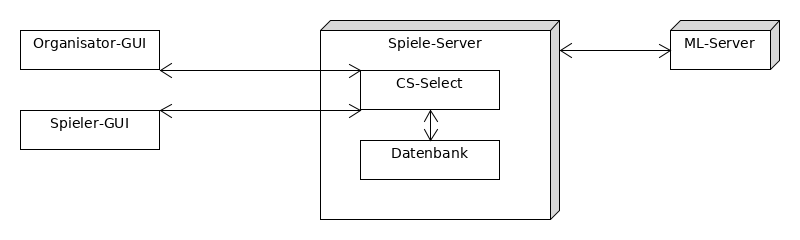
\includegraphics[width=\textwidth]{uml/export/Architektur.png}
    Das \Gls{Organisator}-GUI und das \Gls{Spieler}-GUI laufen in einem \Gls{Webbrowser}.
    Hier interagieren die \Gls{Spieler} und \Glspl{Organisator} mit dem \Gls{Produkt}.
    Der \Gls{Spiel-Server} koordiniert den Spielablauf, speichert Ergebnisse
    in eine Datenbank ab und kommuniziert mit dem \Gls{ML-Server}.
    Die Kommunikation zwischen \Gls{Spiel-Server} und \Gls{ML-Server} wird durch HTTP-Anfragen stattfinden.
    \section{Anwendungsbereiche}
    Das \Gls{Produkt} dient der Verbesserung der Merkmalsauswahl bei Machine-Learning-Prozessen in wissenschaftlichen
    Experimenten beziehungsweise privatwirtschaftlichen Unternehmen durch das \Gls{Domanenwissen} der \Gls{Spieler}.

    \section{Zielgruppen}
    Die Zielgruppen des \Gls{Produkt}s lassen sich in \Glspl{Organisator} und \Glspl{Spieler} unterscheiden.
    Der \Gls{Organisator} möchte eine Verbesserung der Machine-Learning-Prozesse erreichen, indem er das \Gls{Domanenwissen} der \Gls{Spieler} nutzt.
    Die \Gls{Spieler} tragen durch Spielen des \Gls{Produkt}s mit ihrem \Gls{Domanenwissen} zur besseren Merkmalsauswahl bei.


    \section{Betriebsbedingungen}
    Das \Gls{Produkt} ist für die Nutzung in Büroräumlichkeiten mit gewöhnlichen Arbeitsplatzrechnern vorgesehen.

    \chapter{Umgebung}
    Das \Gls{Produkt} läuft auf einem Server, die Nutzung erfolgt an Arbeitsplatzrechnern.

    \section{Software}
    Das \Gls{Produkt} läuft auf Linux ab Kernel Version 4 und Windows 7 oder neuer.
    Serverseitig benötigt das Produkt außerdem eine MYSQL-Datenbank, eine Java-Laufzeitumgebung sowie einen verfügbaren \Gls{ML-Server}.
    Clientseitig wird entweder Google Chrome oder Mozilla Firefox sowie eine funktionierende Internetverbindung vorausgesetzt.

    \section{Hardware}
    Das \Gls{Produkt} läuft auf Server-Computern, das Frontend wird von gewöhnlichen Arbeitsplatzrechnern angesteuert.

    \section{Machine-Learning-Server}
    Bei dem \Gls{ML-Server} handelt es sich um einen Server, der nicht Bestandteil des \Gls{Produkt}s ist, jedoch zur Herstellung der Funktionalität benötigt wird.
    Der \Gls{ML-Server} kommuniziert mit dem \Gls{Produkt} über das Internet mittels einer REST-API.
    Der \Gls{ML-Server} übernimmt das Machine-Learning und stellt die \Glspl{Datensatz} für das \Gls{Spiel} zur Verfügung.
    Der \Gls{ML-Server} unterstützt mindestens die nachfolgenden Anfragen:
    \begin{itemize}
        \item \texttt{GET /features} Liefert einen \Gls{Datensatz} an den \Gls{Spiel-Server}.
        Parameter: \\ Datensatzidentifier %Falsche Silbentrennung
        \item \texttt{GET /score} Bewertet eine Merkmalsauswahl eines \Gls{Spieler}s.
        Gibt eine Zahl zwischen 0 und 1 zurück, die der Güte der Merkmalsauswahl entspricht.
        Parameter: Datensatzidentifier, ausgewählte Merkmale
    \end{itemize}
    
    
    \chapter{Funktionale Anforderungen}
    
    \section{Verwaltung des \Gls{Spiel-Server}s}
    \begin{tabularx}{\linewidth}{@{}>{\bfseries}l@{\hspace{.5em}}X@{}} 
	/F10/ & Konfiguration einer Config-Datei, die dem Aufsetzen des \Gls{Spiel-Server}s dient, durch \Gls{Administrator} \\
	/F20/ & Globales Passwort für \Glspl{Organisator} muss in /F10/ setzbar sein \\
    /F25/ & \Gls{ML-Server} muss in /F10/ setzbar sein
    \end{tabularx}

    \section{Optional: Einfachere Verwaltung des \Gls{Spiel-Server}s}
    \begin{tabularx}{\linewidth}{@{}>{\bfseries}l@{\hspace{.5em}}X@{}} 
	/F30/ & Bei Start des Systems gibt es ein Dialog zur einfacheren Einrichtung \\ %Explizit: Was kann man da machen?
	/F40/ & \Glspl{Spiel} sind aus dem System löschbar \\
    /F45/ & \Glspl{Organisator} sind aus dem System löschbar \\
	/F50/ & \Gls{Spiel-Server} kann vom Terminal aus beendent werden \\
	/F60/ & Kontrollierter Neustart: \Gls{Spiel-Server} behält seinen Zustand über Stoppen und Starten hinweg
    \end{tabularx}
    
    \section{Nutzerverwaltung}
    \begin{tabularx}{\linewidth}{@{}>{\bfseries}l@{\hspace{.5em}}X@{}} 
	/F70/ & Erstregistrierung des \Gls{Organisator}s mit E-Mail und dem in /F20/ global gesetztem Passwort \\
	/F80/ & Anmelden des \Gls{Organisator}s mit E-Mail und Passwort \\
	/F90/ & Erstregistrierung eines \Gls{Spieler}s mit E-Mail und Passwort nach dem Erhalten einer Einladung per E-Mail \\
	/F100/ & Anmelden eines \Gls{Spieler}s mit E-Mail und Passwort \\
    /F110/ & Abmelden von \Gls{Organisator} und \Gls{Spieler}
    \end{tabularx}

    \section{Optional: Zusätzliche Funktionen für die Nutzerverwaltung}
    \begin{tabularx}{\linewidth}{@{}>{\bfseries}l@{\hspace{.5em}}X@{}} 
	/F120/ & Änderung der E-Mail von \Glspl{Nutzer}n \\
	/F130/ & Änderung des Passworts von \Glspl{Nutzer}n \\
	/F140/ & Zurücksetzen des Passworts von \Glspl{Nutzer}n ohne Kenntnis des derzeitigen Passworts \\
    \end{tabularx}
    
    \section{Spielerstellung}
    \begin{tabularx}{\linewidth}{@{}>{\bfseries}l@{\hspace{.5em}}X@{}}
    /F150/ & \Gls{Organisator} kann in Spielerstellungs-GUI \Gls{Spieler} zu einem \Gls{Spiel} einladen, indem er E-Mail-Adresse des \Gls{Spieler}s angibt \\
    /F160/ & Eingeladene \Gls{Spieler} erhalten Einladungs-E-Mail \\
    /F170/ & \Gls{Organisator} muss mindestens einen \Gls{Spielmodus} auswählen \\
    /F180/ & Falls in /F170/ \Gls{Matrix Select} ausgewählt ist, muss \Gls{Organisator} Matrixgröße angeben \\
    /F190/ & \Gls{Organisator} muss Name des Merkmalsdatensatzes angeben \\
    /F200/ & \Gls{Organisator} muss Adresse einer Datenbank angeben \\ %Kann?
    /F210/ & \Gls{Organisator} muss Spieltitel und Spielbeschreibung angeben \\ %Kann?
    /F220/ & \Gls{Organisator} muss aus den folgenden Möglichkeiten mindestens eine auswählen und gegebenenfalls Werte angeben: Ende nach bestimmter Zeit, Ende nach bestimmter Anzahl an Runden, Ende durch Spielabbruch durch Organisator \\
    /F230/ & \Gls{Organisator} kann Spielerstellung abbrechen \\
    /F240/ & \Gls{Organisator} muss Spielerstellung bestätigen \\
    %Kann Organisator mehrere Spielmodi zur Auswahl für Spieler geben
    \end{tabularx}
    
    \section{Optional: Zusätzliche Funktionen bei der Spielerstellung}
    \begin{tabularx}{\linewidth}{@{}>{\bfseries}l@{\hspace{.5em}}X@{}}
    /F250/ & \Gls{Organisator} kann seine \Gls{Spieleinstellungen} aus /F170/-/F220/ speichern \\
    /F260/ & \Gls{Organisator} kann seine gespeicherten \Gls{Spieleinstellungen} aus /F250/ laden und für neue Spielerstellung verwenden\\
    /F270/ & \Gls{Organisator} kann weitere \Gls{Spieler} nach Beginn eines \Gls{Spiel}s einladen \\
    /F280/ & \Gls{Spieler} erhalten über Spieler-GUI eine Benachrichtigung, dass sie eingeladen wurden \\ %Per Mail auch?
	\end{tabularx}
    
    \section{Spielablauf} 
    \begin{tabularx}{\linewidth}{@{}>{\bfseries}l@{\hspace{.5em}}X@{}}
    /F290/ & \Gls{Spieler} kann Einladungen zu \Glspl{Spiel}n annehmen und ablehnen \\
    /F300/ & \Gls{Spieler} sieht in Spieler-Übersichts-GUI alle Spiele, bei denen er die Einladung angenommen hat und welche aktiv sind \\
    /F310/ & \Gls{Spieler} kann \Gls{Spiel} auswählen und spielen, anschließend: \\
    /F320/ & \Gls{Spieler} spielt Runde des entsprechenden \Gls{Spielmodus}, für alle gilt: \\
    /F330/ & \Gls{Spieler} kann \Gls{Merkmal} auswählen \\
    /F340/ & \Gls{Spieler} kann sich zu \Gls{Merkmal} zusätzlich eine Kurzbeschreibung und Grafiken anzeigen lassen \\
    /F350/ & Nach Beenden der Runde sieht der \Gls{Spieler} seine Punktzahl und kann entscheiden, ob er noch eine Runde spielen will \\
	/F360/ & Ein \Gls{Spiel} terminiert nach Erreichen seiner Endbedingungen aus /F220/, danach kann keine Runde mehr gespielt werden \\
    /F370/ & \Gls{Spieler} sieht in seinem GUI aktuelle Runde und Punktestand \\
	/F380/ & \Gls{Organisator} kann sich über aktuellen Status seines \Gls{Spiel}s informieren \\ %Genauer? Gespielte Runden einsehen und so?
    /F390/ & \Gls{Organisator} sieht in /F380/ gespielte Anzahl an bisherigen Runden
    \end{tabularx}
    
    \subsection{\Gls{Binar Select}}
    \begin{tabularx}{\linewidth}{@{}>{\bfseries}l@{\hspace{.5em}}X@{}}
        /F400/ & Eine Runde \Gls{Binar Select} besteht aus genau fünf Vergleichen \\
    	/F410/ & Pro Vergleich werden dem \Gls{Spieler} zufällig immer zwei \Glspl{Merkmal} angezeigt \\
    	/F420/ & \Gls{Spieler} muss eines davon auswählen \\
    	/F430/ & \Gls{Spieler} muss bestätigen, dafür muss er genau ein \Gls{Merkmal} ausgewählt haben \\
    \end{tabularx}

    \subsection{\Gls{Matrix Select}}
    \begin{tabularx}{\linewidth}{@{}>{\bfseries}l@{\hspace{.5em}}X@{}}
        /F440/ & Eine Runde \Gls{Matrix Select} besteht aus genau einer Matrix \\
        /F450/ & Es werden zufällige \Glspl{Merkmal} in einer Matrix angezeigt \\
    	/F460/ & Genau die Anzahl an \Glspl{Merkmal}n, die der \Gls{Organisator} in /F180/ ausgewählt hat, werden angezeigt \\
    	/F470/ & \Gls{Spieler} kann eine Teilmenge an \Glspl{Merkmal} auswählen, jedoch mindestens eines \\ % Wie viele Merkmale maximal? Gibt es Obergrenze?
    	/F480/ & \Gls{Spieler} muss bestätigen, dafür muss er mindestens ein \Gls{Merkmal} ausgewählt haben \\
    \end{tabularx}
	
	\section{Optional: Zusätzliche Funktionen im Spielablauf}
	\begin{tabularx}{\linewidth}{@{}>{\bfseries}l@{\hspace{.5em}}X@{}}
		/F490/ & \Gls{Spieler} kann Runde überspringen, dann: \\
		/F500/ & Von der Gesamtpunktzahl des \Gls{Spieler}s werden 100 Punkte abgezogen, die Gesamtpunktzahl wird aber nicht negativ \\ %100? Kann sie negativ werden?
		/F510/ & \Gls{Spieler} kann ein \Gls{Merkmal} als unwichtig markieren \\
	\end{tabularx}
    
    \section{Spielverwaltung}
	\begin{tabularx}{\linewidth}{@{}>{\bfseries}l@{\hspace{.5em}}X@{}} % Linebreaks in der Tabelle
        /F515/ & \Gls{Organisator} kann ein \Gls{Spiel} vorzeitig beenden \\
        /F517/ & \Glspl{Spiel} können durch \Gls{Organisator} gelöscht werden \\
	\end{tabularx}

	
	\section{Optional: Verbesserung der Merkmalsbereitstellung durch das System}
	\begin{tabularx}{\linewidth}{@{}>{\bfseries}l@{\hspace{.5em}}X@{}}
		/F520/ & Die dem \Gls{Spieler} angezeigten \Glspl{Merkmal} in /F410/ und /F450/ werden nicht zufällig ausgewählt \\
		/F530/ & Selbe Merkmalskombinationen werden nicht mehrfach in einem \Gls{Spiel} angezeigt \\
	\end{tabularx}
	    
    \section{Bewertung der Merkmalsauswahl des \Gls{Spieler}s und Ergebnissicherung}
    \begin{tabularx}{\linewidth}{@{}>{\bfseries}l@{\hspace{.5em}}X@{}}
    /F540/ & Merkmalsauswahl des \Gls{Spieler}s wird per HTTP-Anfrage an \Gls{ML-Server} geschickt \\
    /F550/ & Bei \Gls{Matrix Select} wird in /F540/ die ausgewählte Teilmenge der Vergleiche geschickt \\
    /F560/ & Bei \Gls{Binar Select} wird in /F540/ eine gebündelte Menge der Vergleiche geschickt \\
    /F570/ & Rückmeldung des \Gls{ML-Server}s wird in Rundenpunktzahl (s. /F690/) umgewandelt \\ %Wie? Das wird bei Punktesystem erklärt
    /F580/ & Rundenpunktzahl wird zur Gesamtpunktzahl des \Gls{Spieler}s addiert \\
    /F590/ & Rundendaten\footnote{Ausgewählte Merkmale, Spielername, Zeitpunkt, Rundenanzahl, Vorhersagequalität, Punkte} werden in von Organisator ausgewählte Datenbank gespeichert \\ %Datenbank zu Spiel
    \end{tabularx}
    
    \section{GUI}
    \begin{tabularx}{\linewidth}{@{}>{\bfseries}l@{\hspace{.5em}}X@{}} % Linebreaks in der Tabelle
    /F600/ & \Glspl{Nutzer} haben Zugriff auf die Anmeldungs-GUI in einem \Gls{Webbrowser} \\
    /F610/ & \Glspl{Organisator} erreichen nach erfolgreicher Anmeldung die Organisator-Überschichts-GUI \\
    /F620/ & \Gls{Spieler} erreichen nach erfolgreicher Anmeldung die Spieler-Übersichts-GUI \\
    /F630/ & \Glspl{Organisator} gelangen nach Betätigung der Spielerstellungs-Schaltfläche zur Spielerstellungs-GUI \\
    /F640/ & Nach Beenden der Spielerstellung kehren \Glspl{Organisator} auf die Organisator-Übersichts-GUI zurück \\
    /F650/ & \Gls{Spieler} gelangen nach Betätigung der \enquote{Weiterspielen}-Schaltfläche zur Spiel-GUI \\
    /F660/ & Nach Beenden der Runde kehren \Gls{Spieler} entweder auf die Spieler-Übersichts-GUI oder die Spiel-GUI zurück, je nach Auswahl in /F350/ \\
    /F670/ & Nach Abmeldung kehren \Glspl{Nutzer} auf die Anmeldungs-GUI zurück \\
    \end{tabularx}
        
    \section{Gamification-Elemente} %link?
    \label{sec:Gamification-Elemente}
    \begin{tabularx}{\linewidth}{@{}>{\bfseries}l@{\hspace{.5em}}X@{}}
    /F680/ & Punktesystem für \Gls{Spieler} basierend auf ihren Eingaben: \\
    /F690/ & Der für die Merkmalsauswahl erhaltene Wert des \Gls{ML-Server}s wird mit 100 multipliziert und
        auf die nächstgrößere ganze Zahl aufgerundet \\
    \end{tabularx}

    \section{Optional: Weitere Gamification-Elemente}
    \label{sec:Optionale Gamification-Elemente}
    \begin{tabularx}{\linewidth}{@{}>{\bfseries}l@{\hspace{.5em}}X@{}}
	/F700/ & Leaderboard: Auflistung der \Gls{Spieler} mit den meisten Punkten im Spieler-Übersichts-GUI \\
	/F710/ & \Glspl{Achievement}: Errungenschaften für \Gls{Spieler}, die freigeschaltet werden können, nachdem der \Gls{Spieler} bestimmte Ziele oder Aufgaben erledigt \\
	/F720/ & Auflistung der \Glspl{Achievement} aus /F20/ in Spieler-GUI \\ %in der GUI?
	/F730/ & Daily Challenges: Jeden Tag erhält ein \Gls{Spieler} eine neue Herausforderung, die er abschließen kann, diese gibt 50 zusätzliche Punkte \\
	/F740/ & Streaks: Die Punktezahl der jeweiligen Runde für einen \Gls{Spieler} verdoppelt sich, wenn er drei (oder mehrere) Runden in Folge spielt \\
	/F750/ & Erweitertes Punktesystem: Abschließen von /F710/ gibt je nach Schwierigkeitsgrad der Aufgabe zusätzliche Punkte \\
    \end{tabularx}
    
    \section{Bedienungshilfen}
	\begin{tabularx}{\linewidth}{@{}>{\bfseries}l@{\hspace{.5em}}X@{}}
	/F760/ & Hilfe-Schaltfläche in Organisator-GUIs \\
	/F770/ & Hilfe Schaltfläche in Spieler-GUIs \\
	/F780/ & Wenn der \Gls{Nutzer} mit dem Mauszeiger auf einer Schaltfläche im GUI verweilt, erscheint ein Tooltip \\ %Glossar
	\end{tabularx}


    \section{Sprache} %Kapitelname??
    \begin{tabularx}{\linewidth}{@{}>{\bfseries}l@{\hspace{.5em}}X@{}}
	/F790/ & Bereitstellung eines deutschen Sprachpakets für die GUIs \\ 
    \end{tabularx}


    \section{Optional: Internationalisierung}
    \begin{tabularx}{\linewidth}{@{}>{\bfseries}l@{\hspace{.5em}}X@{}}
	/F800/ & Bereitstellung eines englischen Sprachpakets für die GUIs \\
	/F810/ & Änderung der Sprache für  \Gls{Nutzer} im GUI möglich \\
    \end{tabularx}

    \section{Optional: Unterstützung von mehreren Plattformen}
    \begin{tabularx}{\linewidth}{@{}>{\bfseries}l@{\hspace{.5em}}X@{}}
	/F820/ & Unterstützung von Internet Explorer \\
	/F830/ & Unterstützung von Mobilgeräten mit Responsive-GUIs \\
	/F840/ & Lieferung des \Gls{Spiel-Server}s als Docker-Image \\
	/F850/ & Der \Gls{Spiel-Server} kann auf verschiedenen Ports ausgeführt werden \\
    \end{tabularx}

    %Kapitel Sonstiges, wenn noch irgendwas einfällt?
    %TODO: Abgeschlossene Spiele löschen

    \chapter{Produktdaten}

    \section{Nutzerdaten}
    \begin{tabularx}{\linewidth}{@{}>{\bfseries}l@{\hspace{.5em}}X@{}}
        /D10/ & Über \Gls{Nutzer} sind folgende Daten zu speichern /ND10/:
        \begin{itemize}
              \item E-Mail-Adresse, Nutzername, Punktestand (nur \Gls{Spieler}), Rolle, Passwort (als Hash)
        \end{itemize} \\
        /KD10/ & Über einen \Gls{Spieler} werden außerdem seine \Glspl{Achievement} gespeichert. \\
        /KD20/ & Über einen \Gls{Organisator} werden außerdem seine \Gls{Spieleinstellungen} gespeichert. \\
    \end{tabularx}

    \section{Merkmalsdatensätze}
    \begin{tabularx}{\linewidth}{@{}>{\bfseries}l@{\hspace{.5em}}X@{}}
        /D20/ & Für jeden Merkmalsdatensatz ist zu speichern, solange dieser von mindestens einem \Gls{Spiel} benutzt wird: /ND20/:
        \begin{itemize}
             \item Liste an \Glspl{Merkmal}n mit jeweiligen Grafiken und Beschreibung
        \end{itemize}
    \end{tabularx}

    \section{Spieledaten}
    \begin{tabularx}{\linewidth}{@{}>{\bfseries}l@{\hspace{.5em}}X@{}}
        /D30/ & Für jedes \Gls{Spiel} ist zu speichern /ND30/: 
        \begin{itemize}
             \item \Gls{Organisator}, \Gls{Spieleinstellungen}, \Gls{Spieler}, zugehöriger Merkmalsdatensatz, Spielablauf, also das Ergebnis einzelner Runden			 % zuständiger ML Server?
			 \item Für jede Runde: Ausgewählte \Glspl{Merkmal}, Spielername, Zeitpunkt, Rundenanzahl, Vorhersagequalität, Punkte
		\end{itemize}
    \end{tabularx}

    \section{Administrationsdaten}
    \begin{tabularx}{\linewidth}{@{}>{\bfseries}l@{\hspace{.5em}}X@{}}
        /D40/ & Allgemeines \Gls{Organisator}-Passwort für die Registrierung von neuen \Glspl{Organisator} /F20/
    \end{tabularx}

    \chapter{Nichtfunktionale Anforderungen}

    \begin{tabularx}{\linewidth}{@{}>{\bfseries}l@{\hspace{.5em}}X@{}}
        /NF10/ & Es müssen mindestens 30 \Gls{Spieler} zur gleichen Zeit spielen können.\\
        /NF20/ & Die Wartezeiten auf eine Reaktion des GUIs dürfen nicht länger als zwei Sekunden betragen. \\
	    /NF30/ & Die Anmeldedauer aus /F80/ und /F100/ darf nicht mehr als zwei Sekunden betragen. \\
        /NF40/ & Ein \Gls{Spieler} soll das Ergebnis seiner gespielten Runde innerhalb von zwei Sekunden erhalten. \\
        /NF50/ & Das Design soll modern wirken. \\
        /NF60/ & Der \Gls{ML-Server} soll leicht austauschbar sein. \\
        /NF70/ & Neue \Glspl{Spielmodus} sollen leicht hinzugefügt werden können. \\
        /NF80/ & Neue Spieloberflächen sollen leicht erweiterbar sein. \\
        /NF90/ & Neue Sprachen sollen leicht hinzugefügt werden können. \\
        /NF100/ & Browserkompatibilität: Das \Gls{Produkt} enthält nicht mehr als 0,1\% plattformspezifischer Anweisungen. \\
        /NF110/ & Lizensierung des \Gls{Produkt}s mit MIT-Lizenz.
    \end{tabularx}

    \chapter{Testszenarien}
    \section{Organisation}
    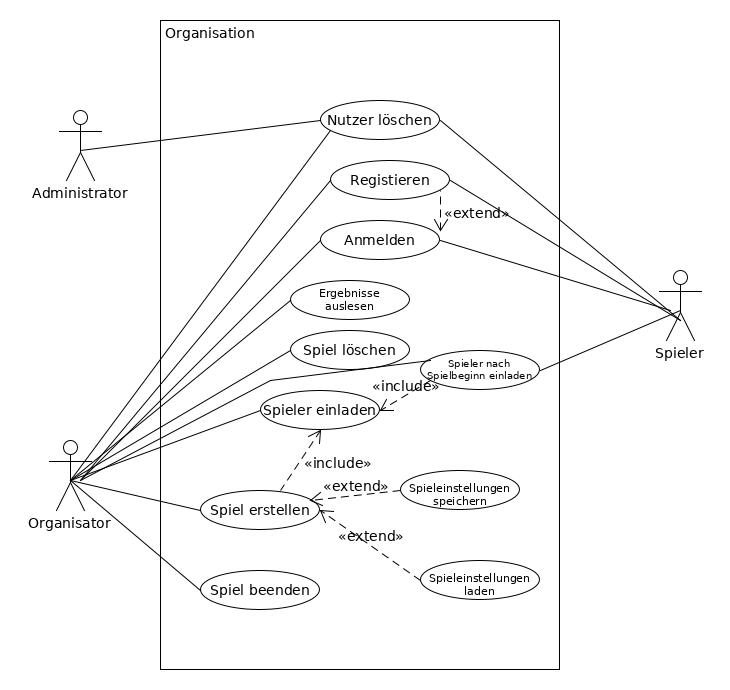
\includegraphics[width=\textwidth]{uml/export/Organisation.png}
    Akteure:
    \begin{itemize}
        \item \Gls{Administrator}
        \item \Gls{Organisator}
        \item \Gls{Spieler}
    \end{itemize}
    \newpage
   \subsection{Spieler registrieren}
    \begin{itemize}
        \item Teilnehmende Akteure: \Gls{Organisator}, \Gls{Spieler}
        \item Eingangsbedingungen: \Gls{Spiel-Server} ist aktiv
        \item Ereignisfluss:
        \begin{itemize}
            \item \Gls{Organisator} lädt den \Gls{Spieler} über das Organisator-GUI ein
            \item Der \Gls{Spieler} klickt auf den Einladungslink in der E-Mail und wird auf die Registrierungsseite weitergeleitet
            \item Der \Gls{Spieler} gibt einen einzigartigen Nutzernamen, seine E-Mail-Adresse sowie ein persönliches Passwort ein und bestätigt
        \end{itemize}
        \item Anforderungen: /F90/
    \end{itemize}

    \subsection{Spieler anmelden}
    \begin{itemize}
        \item Teilnehmende Akteure: \Gls{Spieler}

        \item Eingangsbedingungen: \Gls{Spiel-Server} ist aktiv, \Gls{Spieler} ist registriert

        \item Ereignisfluss:
        \begin{itemize}
            \item \Gls{Spieler} öffnet die Produktwebsite
            \item \Gls{Spieler} wählt die Rolle \enquote{\Gls{Spieler}} in Anmeldungs-GUI aus
            \item \Gls{Spieler} gibt E-Mail und Passwort ein
            \item \Gls{Spieler} klickt auf \enquote{Anmelden}
        \end{itemize}
        \item Anforderungen: /F100/
    \end{itemize}

    \subsection{Spieler abmelden}
    \begin{itemize}
        \item Teilnehmende Akteure: \Gls{Spieler}
        \item Eingangsbedingungen: \Gls{Spiel-Server} ist aktiv, \Gls{Spieler} ist angemeldet
        \item Ereignisfluss:
        \begin{itemize}
            \item \Gls{Spieler} klickt auf Klappmenü
            \item \Gls{Spieler} klickt auf \enquote{Abmelden}
            \item \Gls{Spieler} bestätigt seine Auswahl
        \end{itemize}
        \item Anforderungen: /F110/
    \end{itemize}

    \begin{comment} %% das ist noch nicht in den anforderungen
    \subsection{Spieler löschen}
    \begin{itemize}
        \item Teilnehmende Akteure: \Gls{Administrator}
        \item Eingangsbedingungen: \Gls{Spiel-Server} ist aktiv
        \item Ereignisfluss:
        \begin{itemize}
            \item \Gls{Administrator} loggt sich am Server ein
            \item \Gls{Administrator} führt das \enquote{Löschen}-Kommando mit dem Nutzernamen des zu löschenden \Gls{Spieler}s aus
            \item \Gls{Administrator} bestätigt den Vorgang
        \end{itemize}
    \end{itemize}
    \end{comment}

    \subsection{Organisator registrieren}
    \begin{itemize}
        \item Teilnehmende Akteure: \Gls{Organisator}
        \item Eingangsbedingungen: \Gls{Spiel-Server} ist aktiv, Organisator-Registrierungspasswort ist gesetzt
        \item Ereignisfluss:
        \begin{itemize}
            \item \Gls{Organisator} öffnet die Produktwebsite und klickt auf Registrieren
            \item \Gls{Organisator} gibt einen einzigartigen Nutzernamen, seine E-Mail-Adresse, das Organisator-Registrierungspasswort sowie ein persönliches Passwort ein und bestätigt seine Auswahl
        \end{itemize}
        \item Anforderungen: /F70/
    \end{itemize}

    \subsection{Organisator anmelden}
    \begin{itemize}
        \item Teilnehmende Akteure: \Gls{Organisator}
        \item Eingangsbedingungen: \Gls{Spiel-Server} ist aktiv
        \item Ereignisfluss:
        \begin{itemize}
            \item \Gls{Organisator} öffnet die Produktwebsite
            \item \Gls{Organisator} wählt die Rolle \enquote{\Gls{Organisator}} in Anmeldungs-GUI aus
            \item \Gls{Organisator} gibt E-Mail und Passwort ein
            \item \Gls{Organisator} klickt auf \enquote{Anmelden}-Schaltfläche
        \end{itemize}
        \item Anforderungen: /F80/
    \end{itemize}

    \subsection{Organisator abmelden}
    \begin{itemize}
        \item Teilnehmende Akteure: \Gls{Organisator}
        \item Eingangsbedingungen: \Gls{Spiel-Server} ist aktiv, \Gls{Organisator} ist angemeldet
        \item Ereignisfluss:
        \begin{itemize}
            \item \Gls{Organisator} klickt auf Klappmenü
            \item \Gls{Organisator} klickt auf \enquote{Abmelden}-Schaltfläche
            \item \Gls{Organisator} bestätigt seine Auswahl
        \end{itemize}
        \item Anforderungen: /F110/
    \end{itemize}

    \subsection{Organisator löschen}
    \begin{itemize}
        \item Teilnehmende Akteure: \Gls{Administrator}
        \item Eingangsbedingungen: \Gls{Spiel-Server} ist aktiv, \Gls{Organisator} existiert
        \item Ereignisfluss:
        \begin{itemize}
            \item \Gls{Administrator} loggt sich am Server ein
            \item \Gls{Administrator} führt das \enquote{Löschen}-Kommando mit dem Nutzernamen des zu löschenden \Gls{Organisator}s aus
            \item \Gls{Administrator} bestätigt den Vorgang
        \end{itemize}
        \item \item Anforderungen: /F45/
    \end{itemize}

    \subsection{Spiel erstellen}
    \begin{itemize}
        \item Teilnehmende Akteure: \Gls{Organisator}, \Gls{Spieler}
        \item Eingangsbedingungen: \Gls{Spiel-Server} ist aktiv, \Gls{Organisator} ist angemeldet
        \item Ausgangsaktionen: \Gls{Spiel} starten, \Gls{Spieler} werden eingeladen
        \item Ereignisfluss:
        \begin{itemize}
            \item \Gls{Organisator} klickt auf \enquote{Spiel erstellen}-Schaltfläche
            \item \Gls{Organisator} sucht sich über seine GUI die gewünschten \Gls{Spieleinstellungen} aus
            \item \Gls{Organisator} lädt \Gls{Spieler} über Angabe der E-Mail in einem Textfeld ein
            \item Eingeladene \Gls{Spieler} erhalten Benachrichtigung über Einladung
            \item \Gls{Organisator} bestätigt seine Auswahl und erstellt das Spiel
        \end{itemize}
        \item Anforderungen: /F150/ - /F260/, /F280/, /F290/
    \end{itemize}

    \subsection{Spieler nach Spielbeginn einladen}
    \begin{itemize}
        \item Teilnehmende Akteure: \Gls{Organisator}, \Gls{Spieler}
        \item Eingangsbedingungen: \Gls{Spiel-Server} ist aktiv, \Gls{Spiel} ist gestartet, \Gls{Organisator} ist angemeldet
        \item Ausgangsaktionen: \Gls{Spieler} werden eingeladen
        \item Ereignisfluss:
        \begin{itemize}
            \item \Gls{Organisator} wählt gestartetes \Gls{Spiel} aus der Übersicht
            \item \Gls{Organisator} betätigt \enquote{Einladen}-Schaltfläche
            \item \Gls{Organisator} tippt E-Mails der \Gls{Spieler} in Textfeld ein
            \item \Gls{Organisator} bestätigt seine Auswahl
            \item \Gls{Spieler} erhält Benachrichtigung über die Einladung
        \end{itemize}
        \item Anforderungen: /F270/ - /F290/ 
    \end{itemize}

    \subsection{Spiel vorzeitig beenden}
    \begin{itemize}
        \item Teilnehmende Akteure: \Gls{Organisator}, \Gls{Spieler}
        \item Eingangsbedingungen: \Gls{Spiel} ist aktiv und gestartet, \Gls{Organisator} ist angemeldet
        \item Ausgangsaktionen: \Gls{Spieler} können \Gls{Spiel} nicht mehr spielen %werden sie benachrichtigt?
        \item Ereignisfluss:
        \begin{itemize}
            \item \Gls{Organisator} wählt gestartetes \Gls{Spiel} aus der Übersicht
            \item \Gls{Organisator} betätigt \enquote{Beenden}-Schaltfläche
            \item \Gls{Organisator} bestätigt seine Auswahl
        \end{itemize}
        \item Anforderungen: /F515/
    \end{itemize}

    \subsection{Spiel löschen}
    \begin{itemize}
        \item Teilnehmende Akteure: \Gls{Organisator}
        \item Eingangsbedingungen: \Gls{Spiel-Server} ist aktiv, es existiert bereits ein Spiel, \Gls{Organisator} ist angemeldet
        \item Ausgangsaktionen: \Gls{Spiel} löschen
        \item Ereignisfluss:
        \begin{itemize}
            \item \Gls{Organisator} wählt über seine GUI das zu löschende Spiel
            \item \Gls{Organisator} bestätigt seine Auswahl
        \end{itemize}
        \item Anforderungen: /F517/
    \end{itemize}

    \subsection{Spieleinstellungen speichern}
    \begin{itemize}
        \item Teilnehmende Akteure: \Gls{Organisator}
        \item Eingangsbedingungen: \Gls{Spiel-Server} ist aktiv, \Gls{Organisator} ist angemeldet
        \item Ausgangsaktionen: \Gls{Spieleinstellungen} wiederverwenden
        \item Ereignisfluss:
        \begin{itemize}
            \item \Gls{Organisator} sucht sich über seine GUI das \Gls{Spiel} aus, von dem er die Einstellungen speichern möchte
            \item \Gls{Organisator} wählt die Option \enquote{Spieleinstellungen speichern}
            \item \Gls{Organisator} bestätigt seine Auswahl und speichert die Einstellungen
        \end{itemize}
        \item Anforderungen: /F250/
    \end{itemize}

    \subsection{Spieleinstellungen laden}
    \begin{itemize}
        \item Teilnehmende Akteure: \Gls{Organisator}
        \item Eingangsbedingungen: \Gls{Spiel-Server} ist aktiv, \Gls{Spieleinstellungen} wurden bereits gespeichert, \Gls{Organisator} ist angemeldet
        \item Ausgangsaktionen: \Gls{Spiel} starten
        \item Ereignisfluss:
        \begin{itemize}
            \item \Gls{Organisator} erstellt über seine GUI ein neues Spiel
            \item \Gls{Organisator} wählt für dieses \Gls{Spiel} \enquote{Spieleinstellungen laden}
            \item \Gls{Organisator} sucht sich die bereits gespeicherte \Gls{Spieleinstellungen} heraus
            \item \Gls{Organisator} bestätigt seine Auswahl
        \end{itemize}
        \item Anforderungen: /F260/
    \end{itemize}

 \subsection{Spielzustand auslesen}
	\begin{itemize}
		\item Teilnehmende Akteure: \Gls{Organisator}
		\item Eingangsbedingungen: \Gls{Spiel-Server} ist aktiv, \Gls{Organisator} ist angemeldet
		\item Ereignisfluss:
		\begin{itemize}
			\item \Gls{Organisator} erreicht seine Übersichtsseite
			\item \Gls{Organisator} sieht den Zustand seiner laufenden Spiele
		\end{itemize}
        \item Anforderungen: /F380/
	\end{itemize}

    \section{Spiel}
    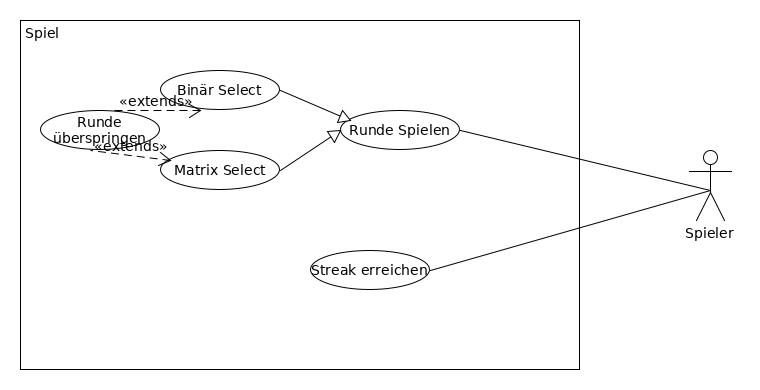
\includegraphics[width=\textwidth]{uml/export/Spiel.png}
    Akteure: 
    \begin{itemize}
    \item \Gls{Spieler}
    \end{itemize}

    \subsection{Einladung zu Spiel annehmen}
    \begin{itemize}
        \item Teilnehmende Akteure: \Gls{Spieler}

        \item Eingangsbedingungen: \Gls{Spiel-Server} ist aktiv, Spieler wurde von \Gls{Organisator} zu einem Spiel eingeladen
        \item Ausgangsaktion: \Gls{Spieler} kann \Gls{Spiel} spielen
        \item Ereignisfluss:\\
        Option 1: 
        Eingangsbedingung: \Gls{Spieler} ist angemeldet
        \begin{itemize}
            \item \Gls{Spieler} klickt auf die \enquote{Ja}-Schaltfläche im Benachrichtigungsfeld der Spieler-GUI
            \item \Gls{Spieler} bestätigt seine Auswahl
            \item Die Benachrichtigung wird vom \Gls{Spiel-Server} gelöscht
            \item \Gls{Spieler} kann an \Gls{Spiel} teilnehmen
        \end{itemize}
        Option 2: 
        \begin{itemize}
            \item \Gls{Spieler} erhält E-Mail mit Einladung und Einladungslink
            \item \Gls{Spieler} klickt auf den Einladungslink
            \item Die Benachrichtigung wird vom \Gls{Spiel-Server} gelöscht
            \item \Gls{Spieler} kann an \Gls{Spiel} teilnehmen
        \end{itemize}

        \item Anforderung: /F290/
    \end{itemize}

    \subsection{Runde spielen: Matrix Select}
    \begin{itemize}
    	\item Teilnehmende Akteure: \Gls{Spieler}

    	\item Eingangsbedingungen: \Gls{Spiel-Server} ist aktiv, \Gls{Spieler} hat offenes \Gls{Spiel} des \Gls{Spielmodus} Matrix Select, \Gls{Spieler} ist angemeldet
        \item Ausgangsaktion: System gibt Spieler die erreichte Punktzahl an
    	\item Ereignisfluss:
    	\begin{itemize}
    		\item \Gls{Spieler} klickt auf ein \Gls{Merkmal} und sieht Merkmalsgraphen und Merkmalsbeschreibung
    		\item \Gls{Spieler} wählt mehrere \Glspl{Merkmal} aus
    		\item \Gls{Spieler} klickt auf Schaltfläche, um Auswahl zu bestätigen
    	\end{itemize}
        \item Anforderungen: /F400/ - /F430/
    \end{itemize}
	
	\subsection{Runde spielen: Binär Select}
	\begin{itemize}
		\item Teilnehmende Akteure: \Gls{Spieler}

		\item Eingangsbedingungen: \Gls{Spiel-Server} ist aktiv, \Gls{Spieler} hat offenes \Gls{Spiel} des \Gls{Spielmodus} Binär Select, \Gls{Spieler} ist angemeldet
        \item Ausgangsaktion: System gibt \Gls{Spieler} die erreichte Punktzahl an
		\item Ereignisfluss:
		\begin{itemize}
			\item \Gls{Spieler} klickt auf ein \Gls{Merkmal} und sieht Merkmalsgraphen und Merkmalsbeschreibung
			\item \Gls{Spieler} wählt eines der beiden \Glspl{Merkmal} aus
			\item \Gls{Spieler} klickt auf Schaltfläche, um Auswahl zu bestätigen
            \item Wiederhole Ereignisfluss fünf Mal
		\end{itemize}
        \item Anforderungen: /F440/ - /F480/
	\end{itemize}

	\subsection{Auswahl überspringen}
	\begin{itemize}
		\item Teilnehmende Akteure: \Gls{Spieler}
		\item Eingangsbedingungen: \Gls{Spiel-Server} ist aktiv, \Gls{Spieler} ist angemeldet und hat offenes Spiel
        \item Ausgangsaktionen: \begin{itemize}
					\item Falls Spielmodus \Gls{Matrix Select} oder \Gls{Binar Select} im 5. Vergleich: Spieler verliert 100 Punkte, System gibt \Gls{Spieler} die erreichte Punktzahl an
					\item Falls Spielmodus \Gls{Binar Select} vor dem 5. Vergleich: Spieler erreicht nächsten Vergleich, Spieler verliert 100 Punkte
					\end{itemize}
		\item Ereignisfluss:
		\begin{itemize}
			\item \Gls{Spieler} klickt auf \enquote{Weiterspielen}-Schaltfläche
			\item \Gls{Spieler} erreicht Spiel-GUI
			\item \Gls{Spieler} klickt \enquote{Auswahl Überspringen}-Schaltfläche und bestätigt seine Auswahl
		\end{itemize}
        \item Anforderungen: /F490/, /F500/
	\end{itemize}
     
    \subsection{Streak erreichen}\footnote{Zur Erklärung von Streak siehe \fref{fig:Streak_State}}
    \begin{itemize}
        \item Teilnehmende Akteure: \Gls{Spieler}
        \item Eingangsbedingungen: \Gls{Spieler} spielt eine Runde
        \item Ausgangsaktionen: \Gls{Spieler} erhält doppelte Punkte für seine Runde
        \item Ereignisfluss:
        \begin{itemize}
            \item \Gls{Spieler} spielt n Runden am Stück, um eine Streak zu erreichen
            \item System teilt dem \Gls{Spieler} mit, dass er eine Streak erreicht hat
        \end{itemize}
        \item Anforderungen: /F740/
    \end{itemize}
    
    \section{Spieler-Übersicht}
    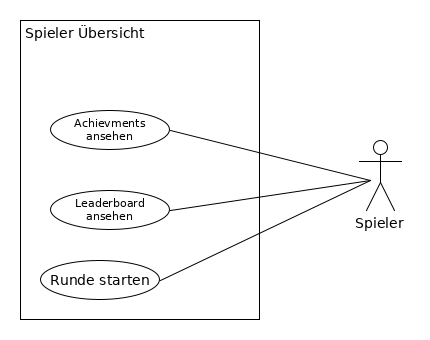
\includegraphics[width=\textwidth]{uml/export/Spieler_Ubersicht.png}
    Akteure: 
    \begin{itemize}
    \item \Gls{Spieler}
    \end{itemize}

    \subsection{Achievements ansehen}
    \begin{itemize}
        \item Teilnehmende Akteure: \Gls{Spieler}
        \item Eingangsbedingungen: \Gls{Spiel-Server} ist aktiv, \Gls{Spieler} ist angemeldet
        \item Ereignisfluss:
        \begin{itemize}
            \item \Gls{Spieler} erreicht seine Spieler-Übersichts-GUI
            \item \Gls{Spieler} klickt auf die Achievements-Schaltfläche %TODO Wo werden die angezeigt
            \item \Gls{Spieler} erhält Auflistung der Achievements
            \item \Gls{Spieler} schaut seine Achievements an
        \end{itemize}
        \item Anforderungen: /F710/
    \end{itemize}

    \subsection{Leaderboard ansehen}
    \begin{itemize}
        \item Teilnehmende Akteure: \Gls{Spieler}
        \item Eingangsbedingungen: \Gls{Spiel-Server} ist aktiv, \Gls{Spieler} ist angemeldet
        \item Ereignisfluss:
        \begin{itemize}
            \item \Gls{Spieler} erreicht seine Spieler-Übersichts-GUI
            \item \Gls{Spieler} sieht dort in einer Tabelle die \Gls{Spieler} mit den meisten Punkten
        \end{itemize}
        \item Anforderungen: /F700/
    \end{itemize}

    \newpage
    \section{Administration}
    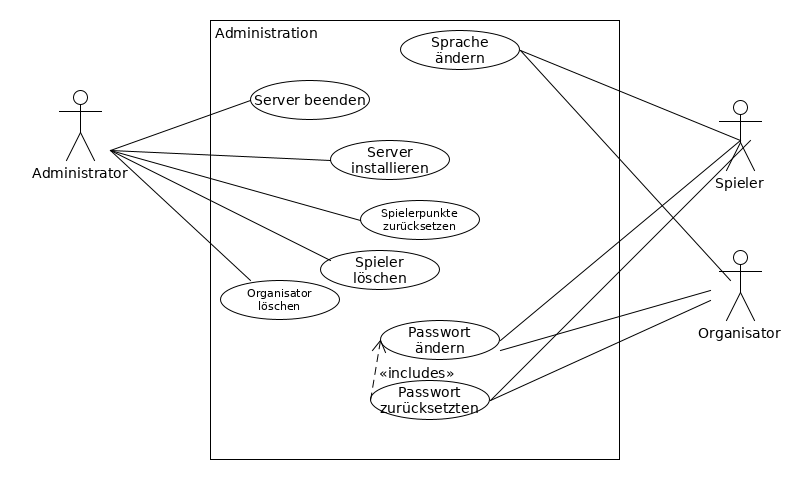
\includegraphics[width=\textwidth]{uml/export/Administration.png}

    \subsection{Sprache ändern}
    \begin{itemize}
    \item Teilnehmende Akteure: \Gls{Spieler}, \Gls{Organisator}
    \item Eingangsbedingungen: \Gls{Spiel-Server} ist aktiv, \Gls{Spieler} oder \Gls{Organisator} ist angemeldet
    \item Ereignisfluss:
        \begin{itemize}
            \item \Gls{Organisator} oder \Gls{Spieler} erreicht über sein Klappmenü seine Einstellungen
            \item \Gls{Organisator} oder \Gls{Spieler} wählt \enquote{Sprache ändern} aus
            \item \Gls{Organisator} oder \Gls{Spieler} wählt eine der verfügbaren Sprachen
            \item \Gls{Organisator} oder \Gls{Spieler} bestätigt seine Auswahl
        \end{itemize}
        \item Anforderungen: /F790/ - /F810/
    \end{itemize}

    \subsection{Server beenden}
    \begin{itemize}
        \item Teilnehmende Akteure: \Gls{Administrator}
        \item Eingangsbedingungen: \Gls{Spiel-Server} ist aktiv
        \item Ereignisfluss: \Gls{Administrator} führt \texttt{tomcat/bin/shutdown.sh} (Linux \& Mac) bzw.  \texttt{tomcat\textbackslash bin\textbackslash shutdown.bat} (Windows)
        \item Anforderungen: /F50/
    \end{itemize}

    \subsection{Passwort ändern}
    \begin{itemize}
    \item Teilnehmende Akteure: \Gls{Spieler}, \Gls{Organisator}
    \item Eingangsbedingungenn: \Gls{Spiel-Server} ist aktiv, \Gls{Spieler} oder \Gls{Organisator} ist angemeldet
    \item Ereignisfluss:
        \begin{itemize}
            \item \Gls{Organisator} oder \Gls{Spieler} erreicht über sein Klappmenü seine Einstellungen
            \item \Gls{Organisator} oder \Gls{Spieler} klickt auf \enquote{Passwort ändern}
            \item \Gls{Organisator} oder \Gls{Spieler} gibt sein aktuelles sowie sein neues gewünschtes Passwort ein
            \item \Gls{Organisator} oder \Gls{Spieler} bestätigt seine Auswahl
        \end{itemize}
        \item Anforderungen: /F130/
    \end{itemize}

    \subsection{Passwort zurücksetzen}
    \begin{itemize}
        \item Teilnehmende Akteure: \Gls{Spieler}, \Gls{Organisator}
        \item Eingangsbedingungen: \Gls{Spiel-Server} ist aktiv, \Gls{Spieler} oder \Gls{Organisator} ist in Anmelde-GUI
        \item Ereignisfluss:
        \begin{itemize}
            \item \Gls{Organisator} oder \Gls{Spieler} klickt in Anmeldungs-GUI auf \enquote{Passwort vergessen?}
            \item \Gls{Organisator} oder \Gls{Spieler} erhält per E-Mail ein neues temporäres Passwort
            \item \Gls{Organisator} oder \Gls{Spieler} meldet sich mit dem neuen Passwort an
        \end{itemize}
        \item Anforderungen: /F140/
    \end{itemize}

    \subsection{Hilfe-Schaltfläche verwenden}
    \begin{itemize}
        \item Teilnehmende Akteure: \Gls{Spieler}, \Gls{Organisator}
        \item Eingangsbedingungen: \Gls{Spieler} oder \Gls{Organisator} benötigt Hilfe mit dem Produkt
        \item Ausgangsaktionen: System zeigt dem Akteur die relevante Hilfe-Seite
        \item Ereignisfluss:
            \begin{itemize}
                \item \Gls{Spieler} oder \Gls{Organisator} klickt in seinem GUI auf die Hilfe-Schaltfläche(oben rechts)
            \end{itemize}
        \item Anforderungen: /F760/
    \end{itemize}

    %TODO: Ausführung auf verschiedenem Ports

    \chapter{Dynamische Modelle}
    \section{Zustandsdiagramme}
    \subsection{Streak}
    \label{fig:Streak_State}
    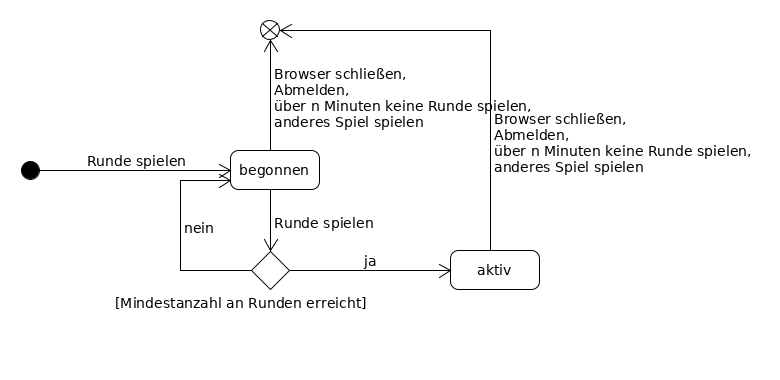
\includegraphics[width=\textwidth]{uml/export/Streak_Zustand.png}
    Die Zustände, die eine Streak haben kann. Eine Streak ist immer auf einen \Gls{Spieler} beschränkt.
    Zustandsbeschreibung:
    \begin{itemize}
    \item begonnen: Eine angefangene Streak, die noch nicht lang genug ist, um für den \Gls{Spieler} eine erhöhte Punktzahl zu erreichen.
    \item aktiv: Die Streak ist lang genug. In diesem Zustand erhält der \Gls{Spieler} doppelt so viele Punkte.
    \end{itemize}
    \subsection{Spiel}
    \label{fig:Spiel_State}
    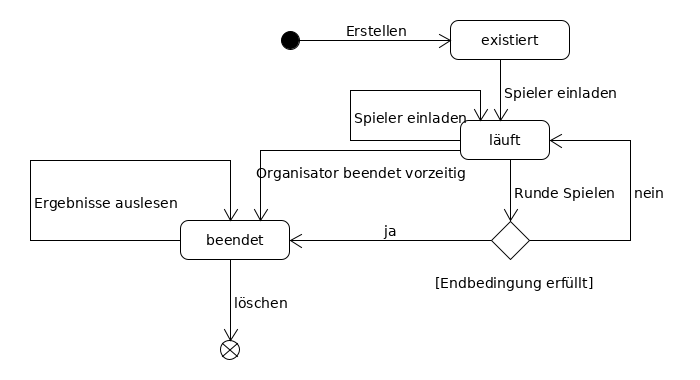
\includegraphics[width=\textwidth]{uml/export/Spiel_Zustand.png}
    Die Zustände, die ein \Gls{Spiel} von der Erstellung bis zum Beenden haben kann.
    Zustandsbeschreibung:
    \begin{itemize}
    \item existiert: Das \Gls{Spiel} existiert, besitzt also einen Datensatz, Endbedingungen und Spielmodus. Es sind aber noch keine \Gls{Spieler} eingeladen, also kann es nicht gespielt werden.
    \item läuft: Das \Gls{Spiel} kann von \Gls{Spieler}n gespielt werden.
    \item beendet: Das \Gls{Spiel} wurde beendet. Kein \Gls{Spieler} kann mehr eine Runde spielen. Die Ergebnisse können aber noch ausgelesen werden.
    \end{itemize}
    \subsection{Achievements}
    \label{fig:Achievment_State}
    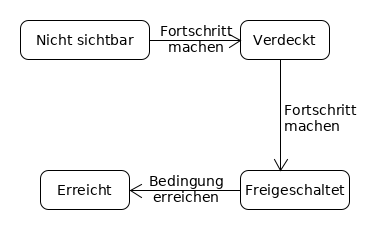
\includegraphics[width=\textwidth]{uml/export/Achievment_State.png}
    Die Zustände, die ein \Gls{Achievement} von \enquote{\Gls{Spieler} kennt das \Gls{Achievement} nicht} bis zu \enquote{\Gls{Spieler} hat das \Gls{Achievement} erreicht}.
    \begin{itemize}
    \item Nicht sichtbar: \Gls{Spieler} weiß nicht, dass das \Gls{Achievement} existiert.
    \item Verdeckt: \Gls{Spieler} weiß, dass dieses \Gls{Achievement} existiert, aber weiß nicht, was er tun muss, um es zu erreichen.
    \item Freigeschaltet: Die Bedingungen für das Erreichen dieses \Gls{Achievement}s sind dem \Gls{Spieler} bekannt.
    \item Erreicht: Der \Gls{Spieler} hat die Bedingungen für das Erreichen dieses \Gls{Achievement}s erfüllt.
    \end{itemize}
    

    \chapter{Benutzerschnittstelle}

    \section{Anmeldung}
    \centering
    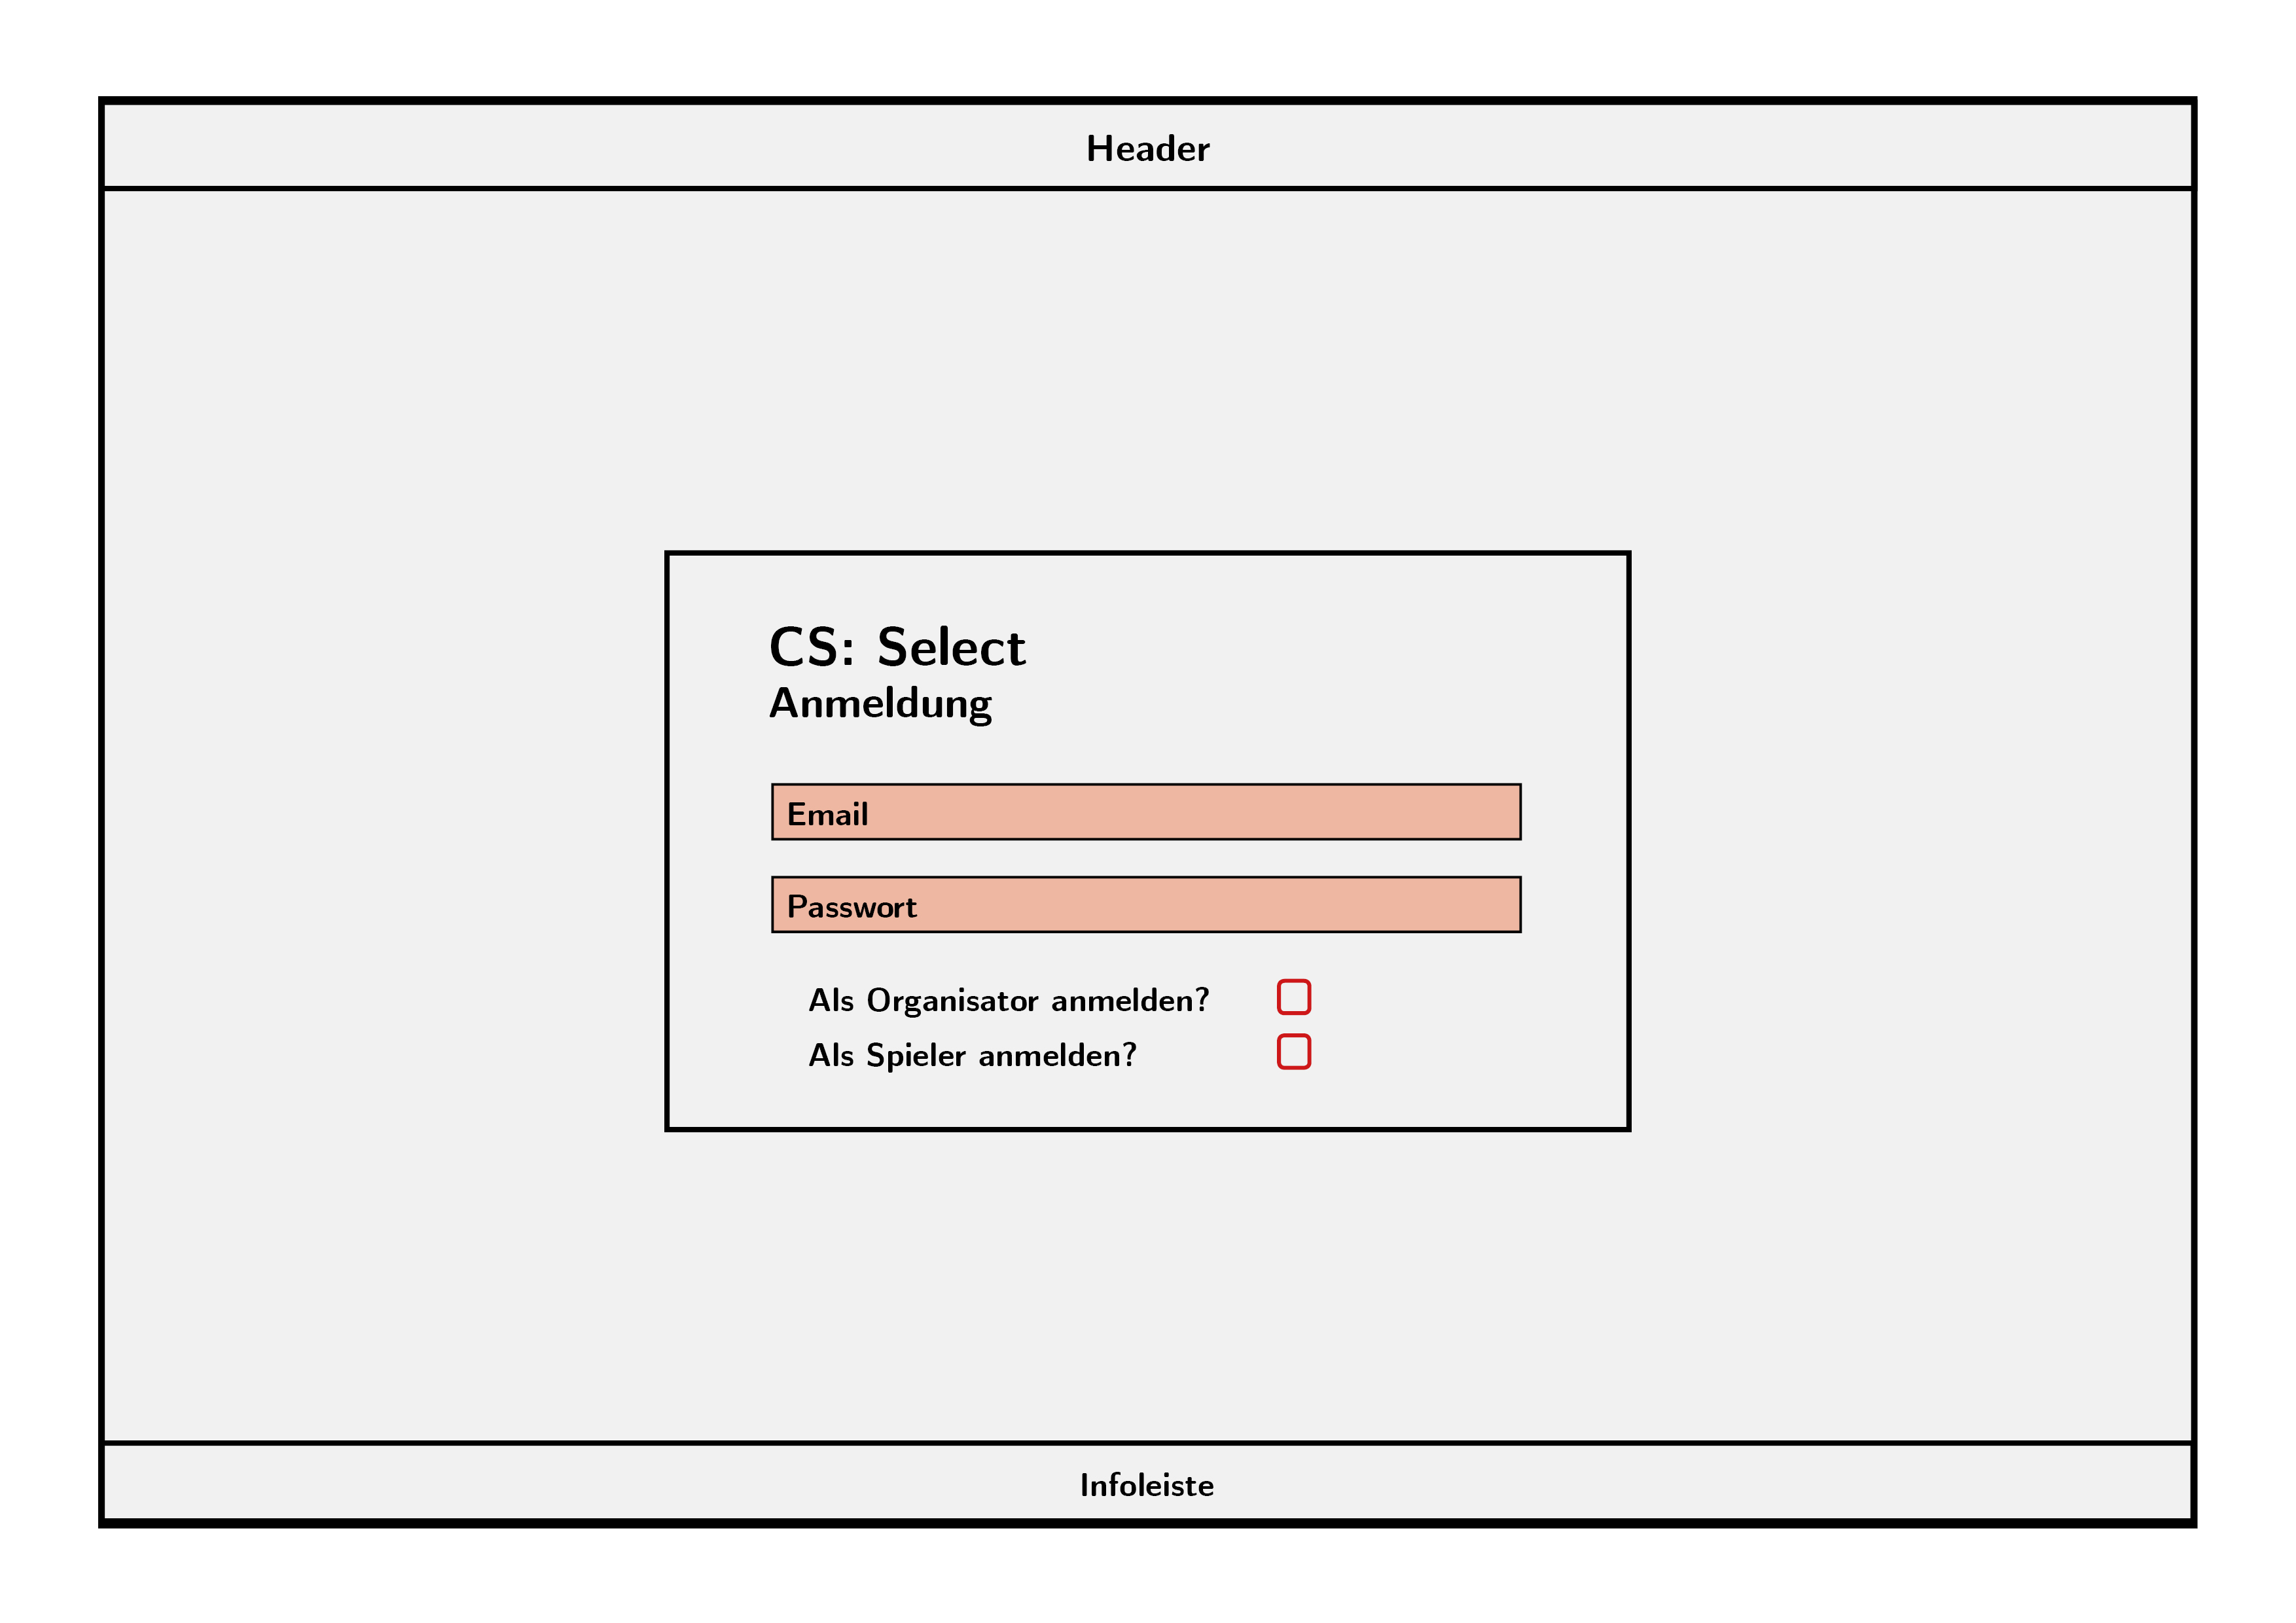
\includegraphics[width=\textwidth]{../pictures/Anmeldung.jpg}
    \subsection{Anmeldung (responsive)}
    \centering
    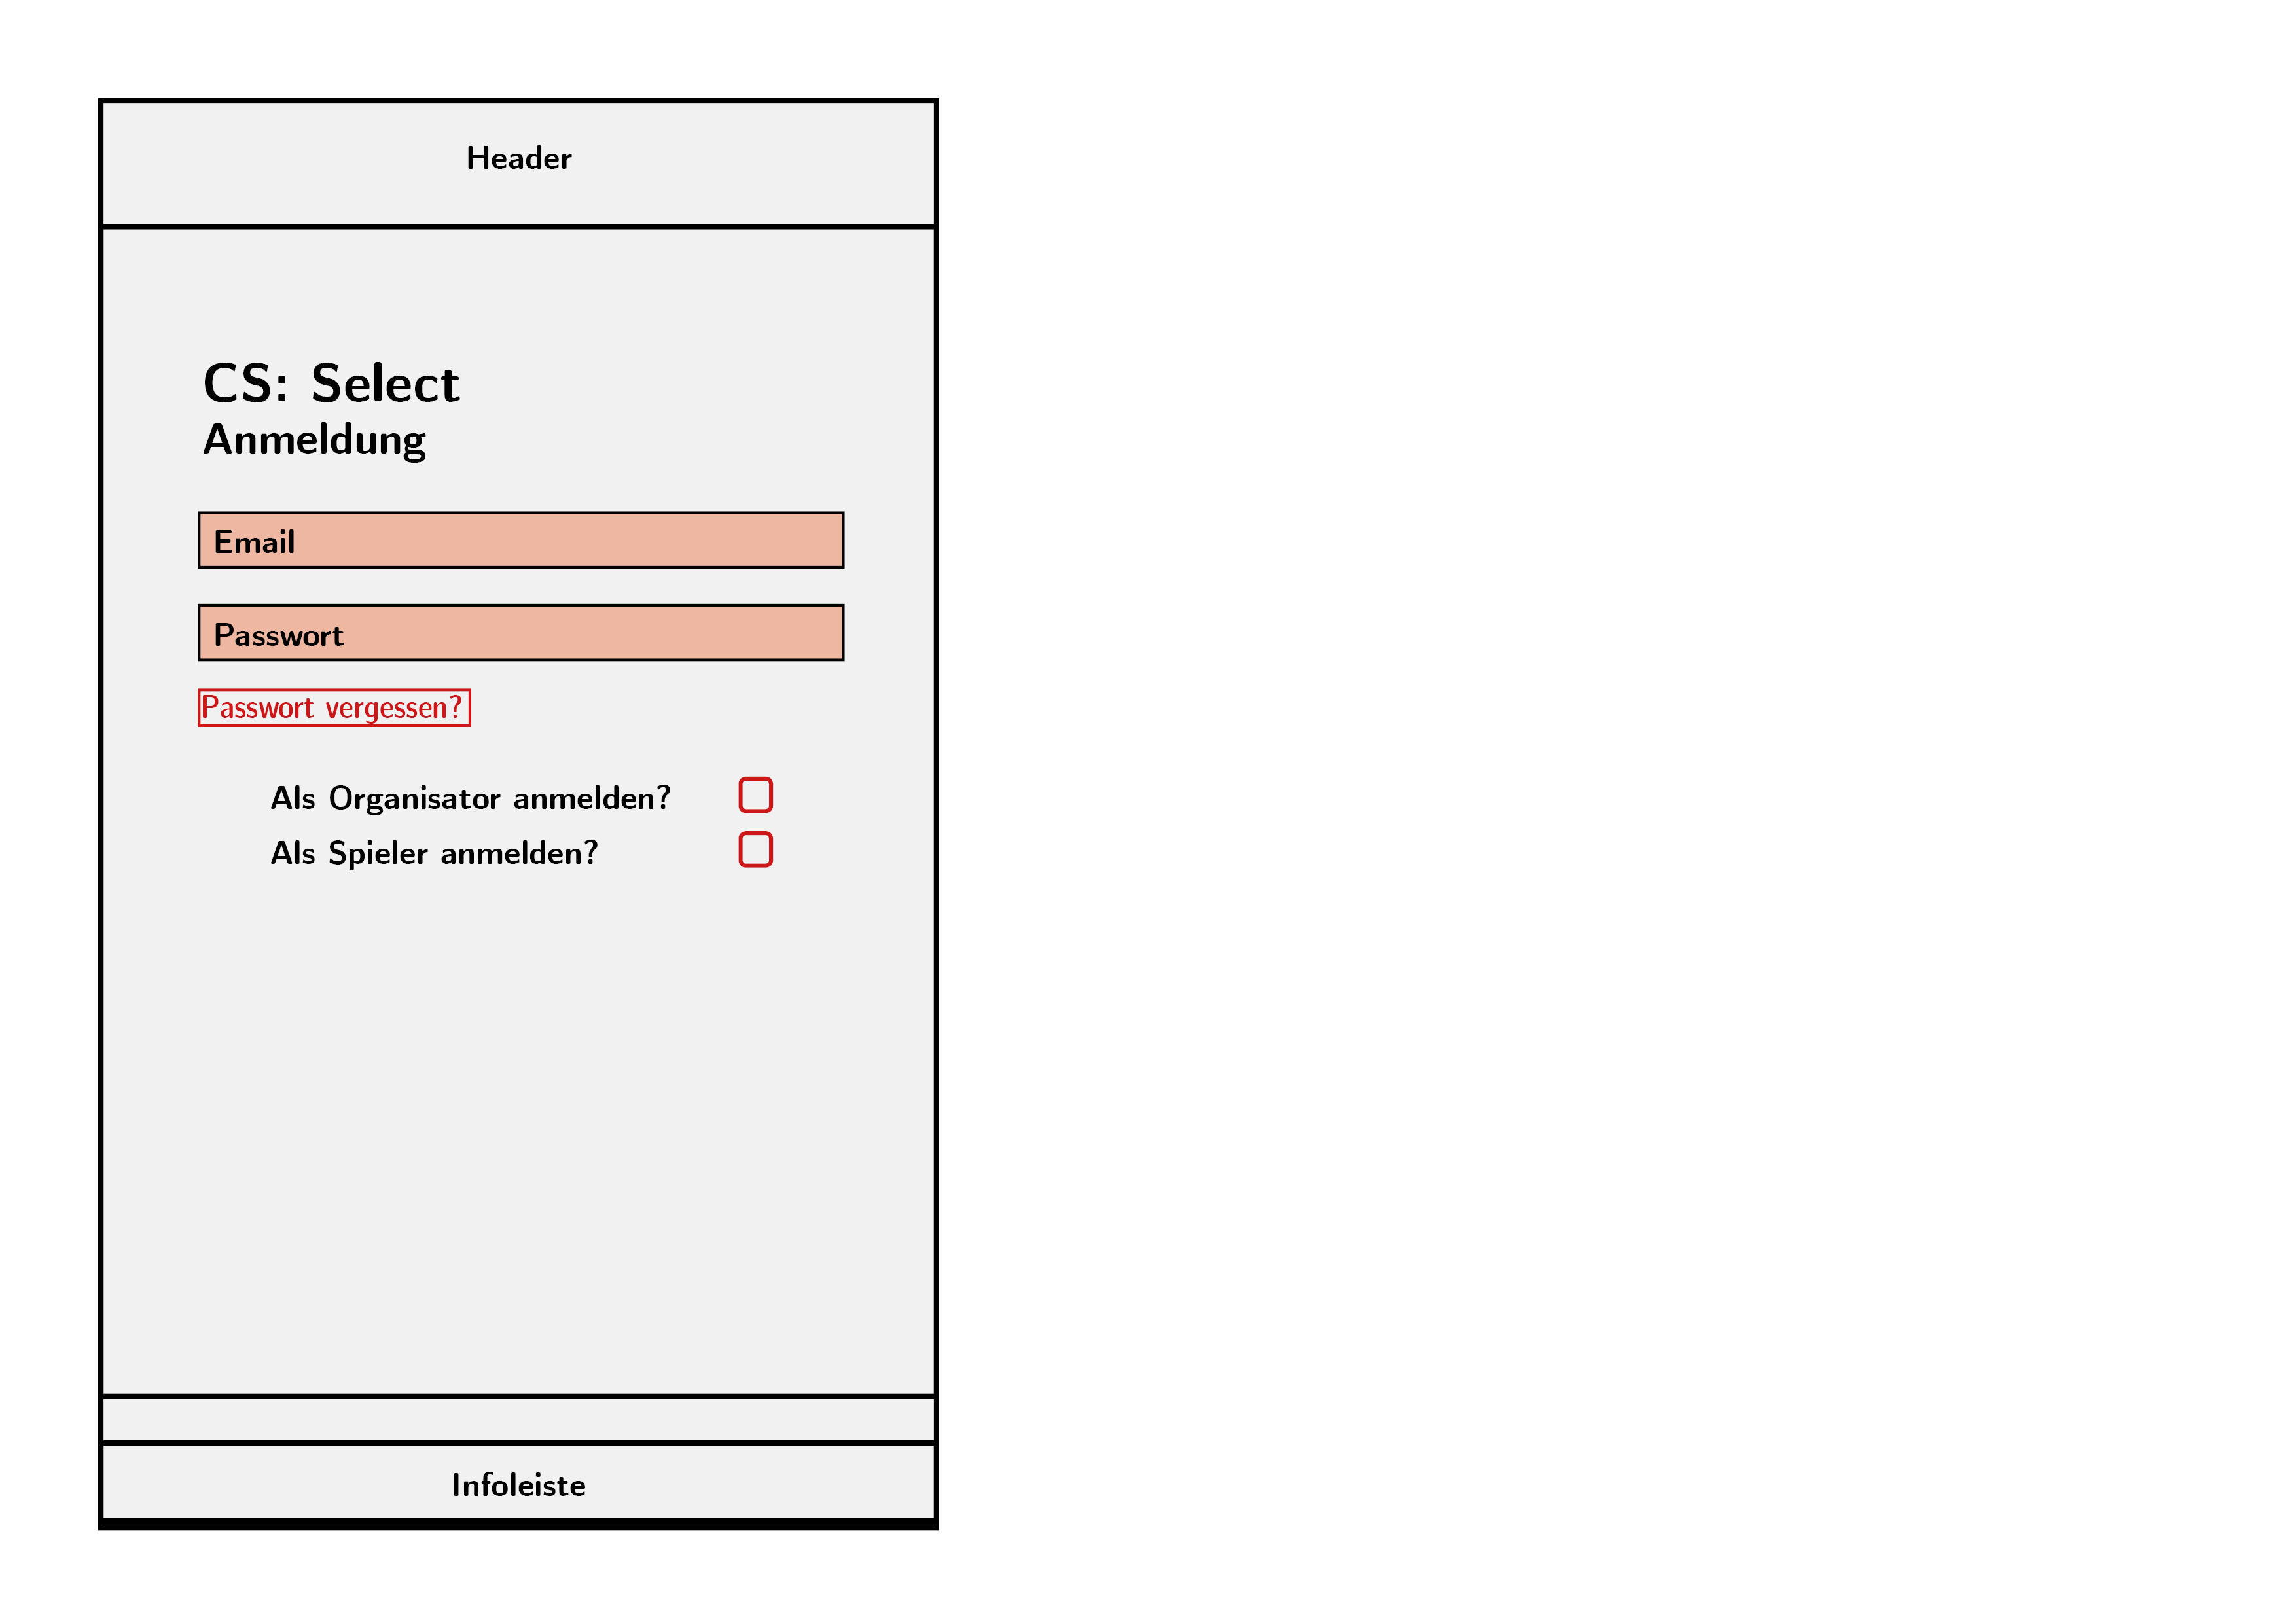
\includegraphics[width=\textwidth]{../pictures/Anmeldung_responsive.jpg}\\

    \section{Organisator-Start}
    \centering
    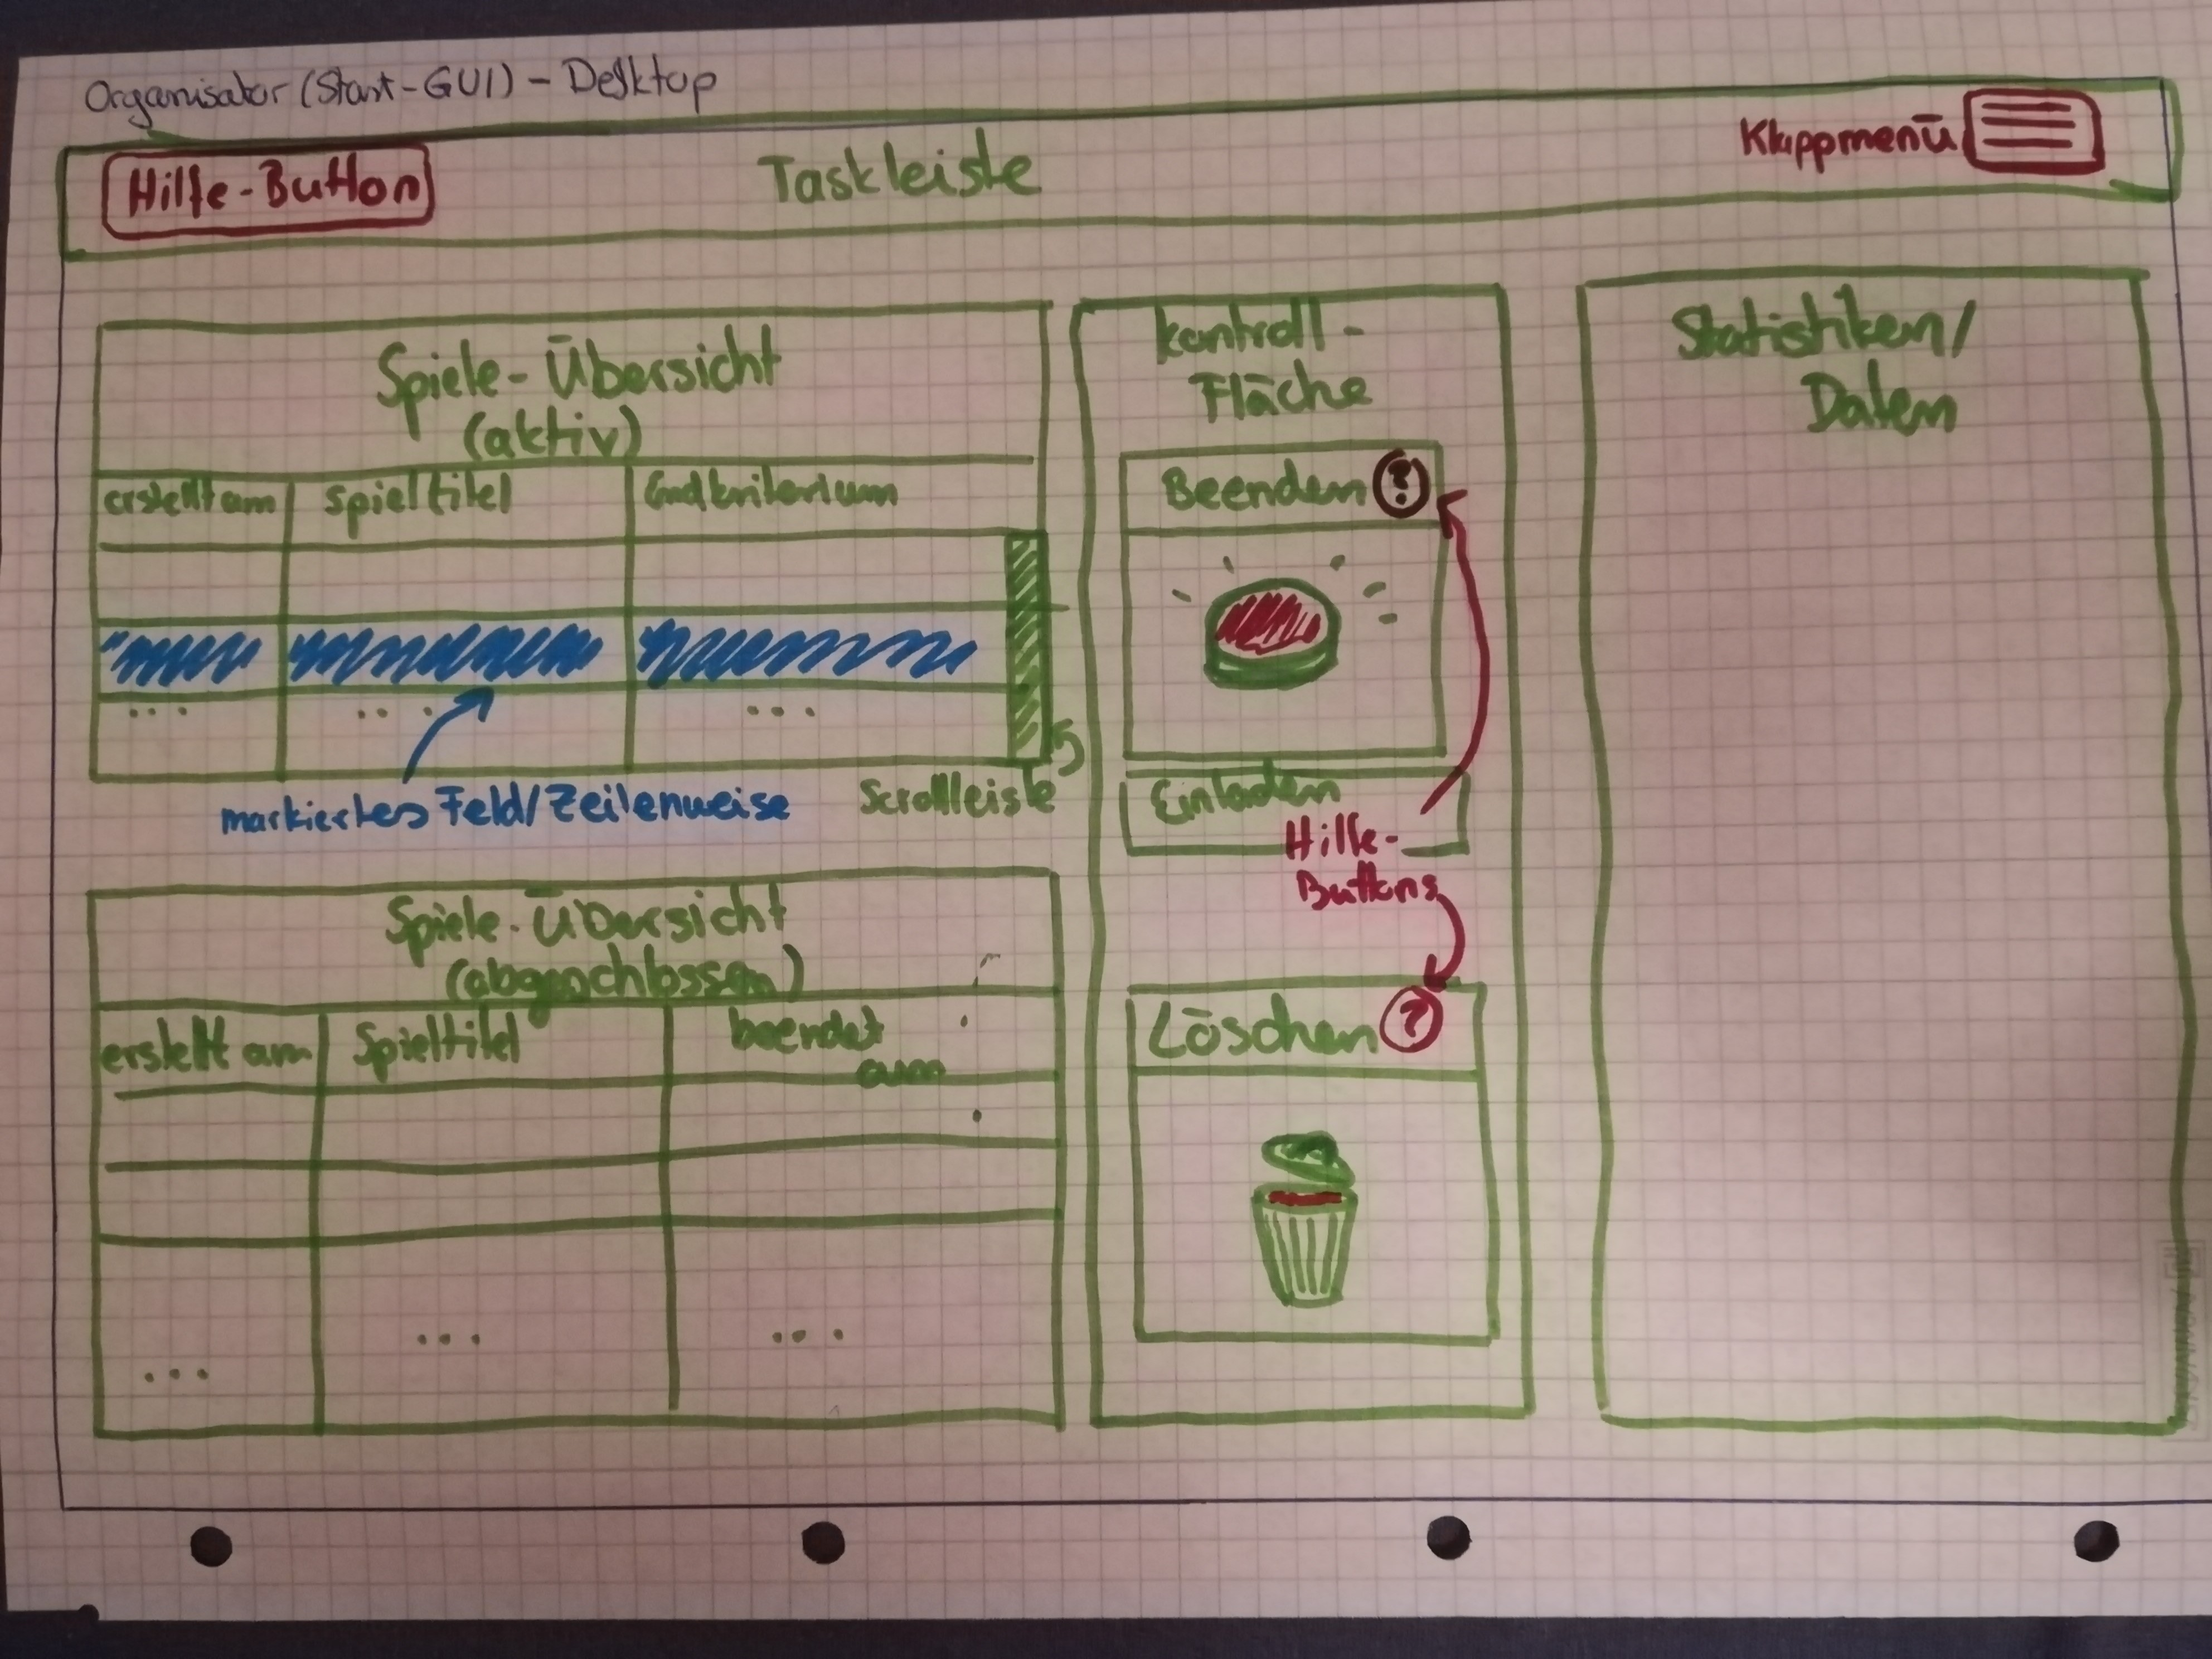
\includegraphics[width=\textwidth]{../pictures/2_Organisator.jpg}

    \subsection{Organisator-Start (responsive)}
    \centering
    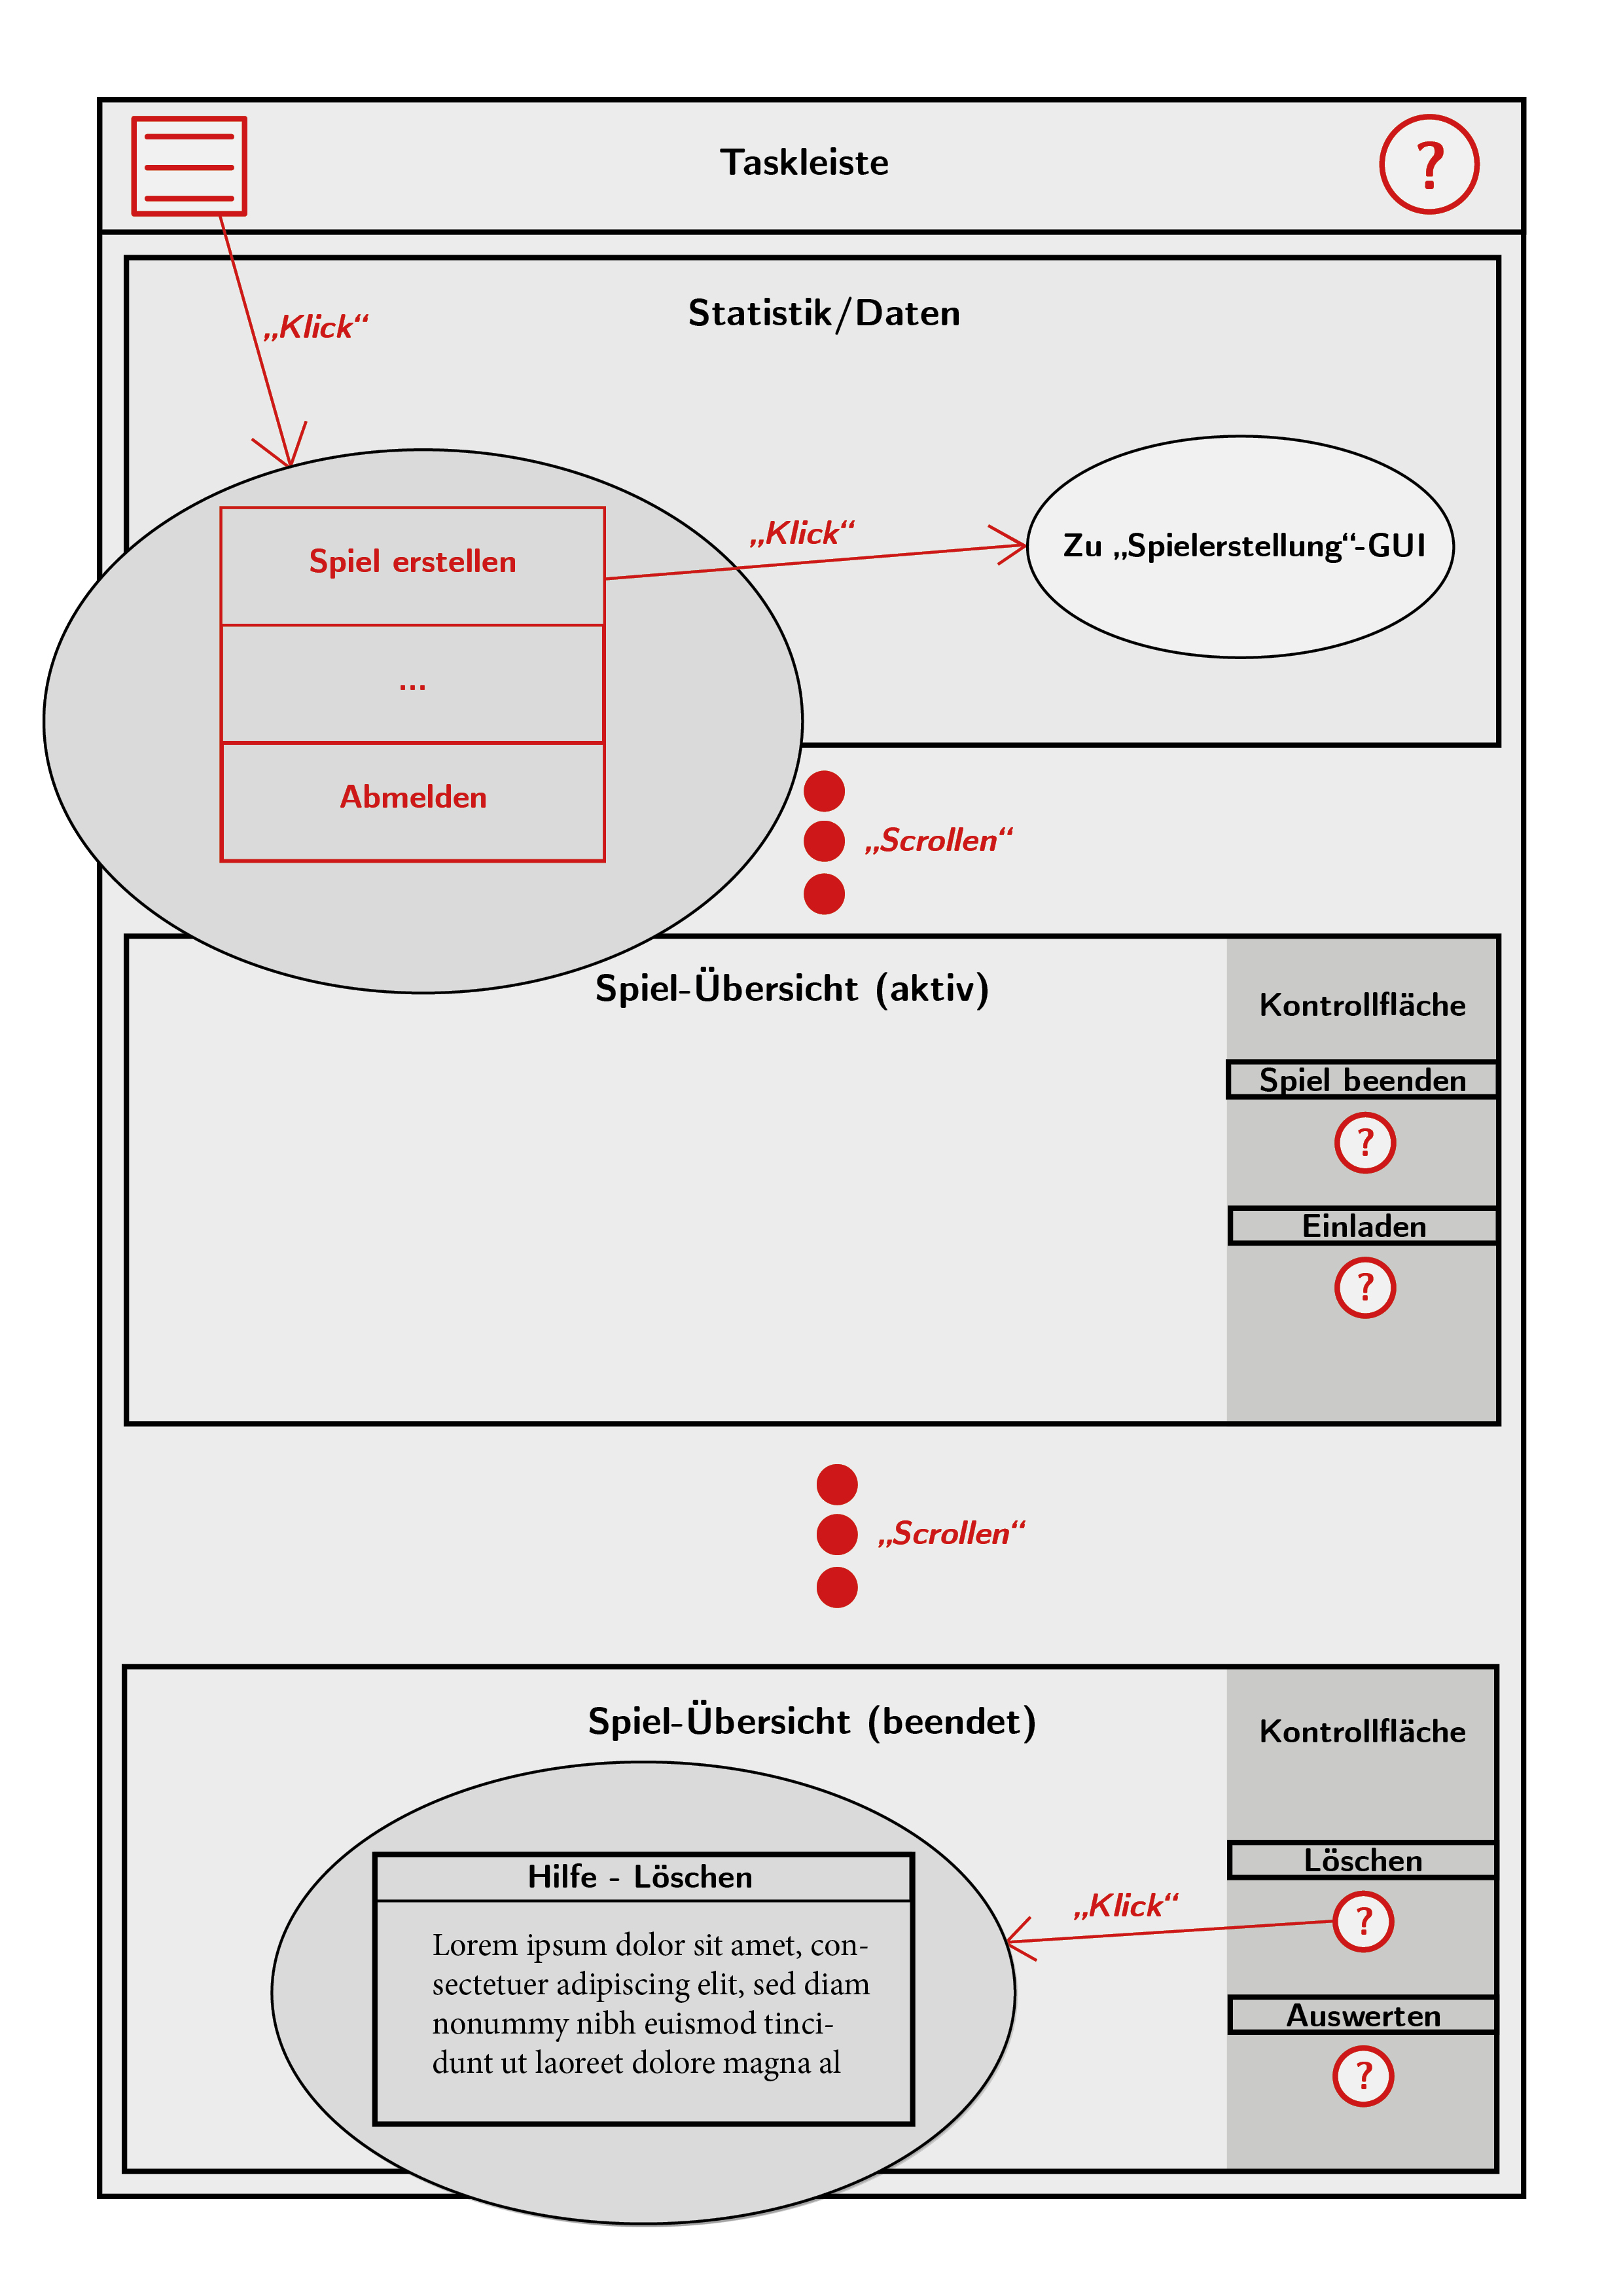
\includegraphics[width=13cm]{../pictures/3_Organisator(responsive).jpg}\\
    In den weiteren Darstellungen werden keine responsiven Darstellungen gezeigt. Die zwei bereits gezeigten Darstellungen dienen als anschauliches Beispiel für
    die responsive Darstellung einer Benutzerschnittstelle.

    \section{Spielerstellung}
    \centering
    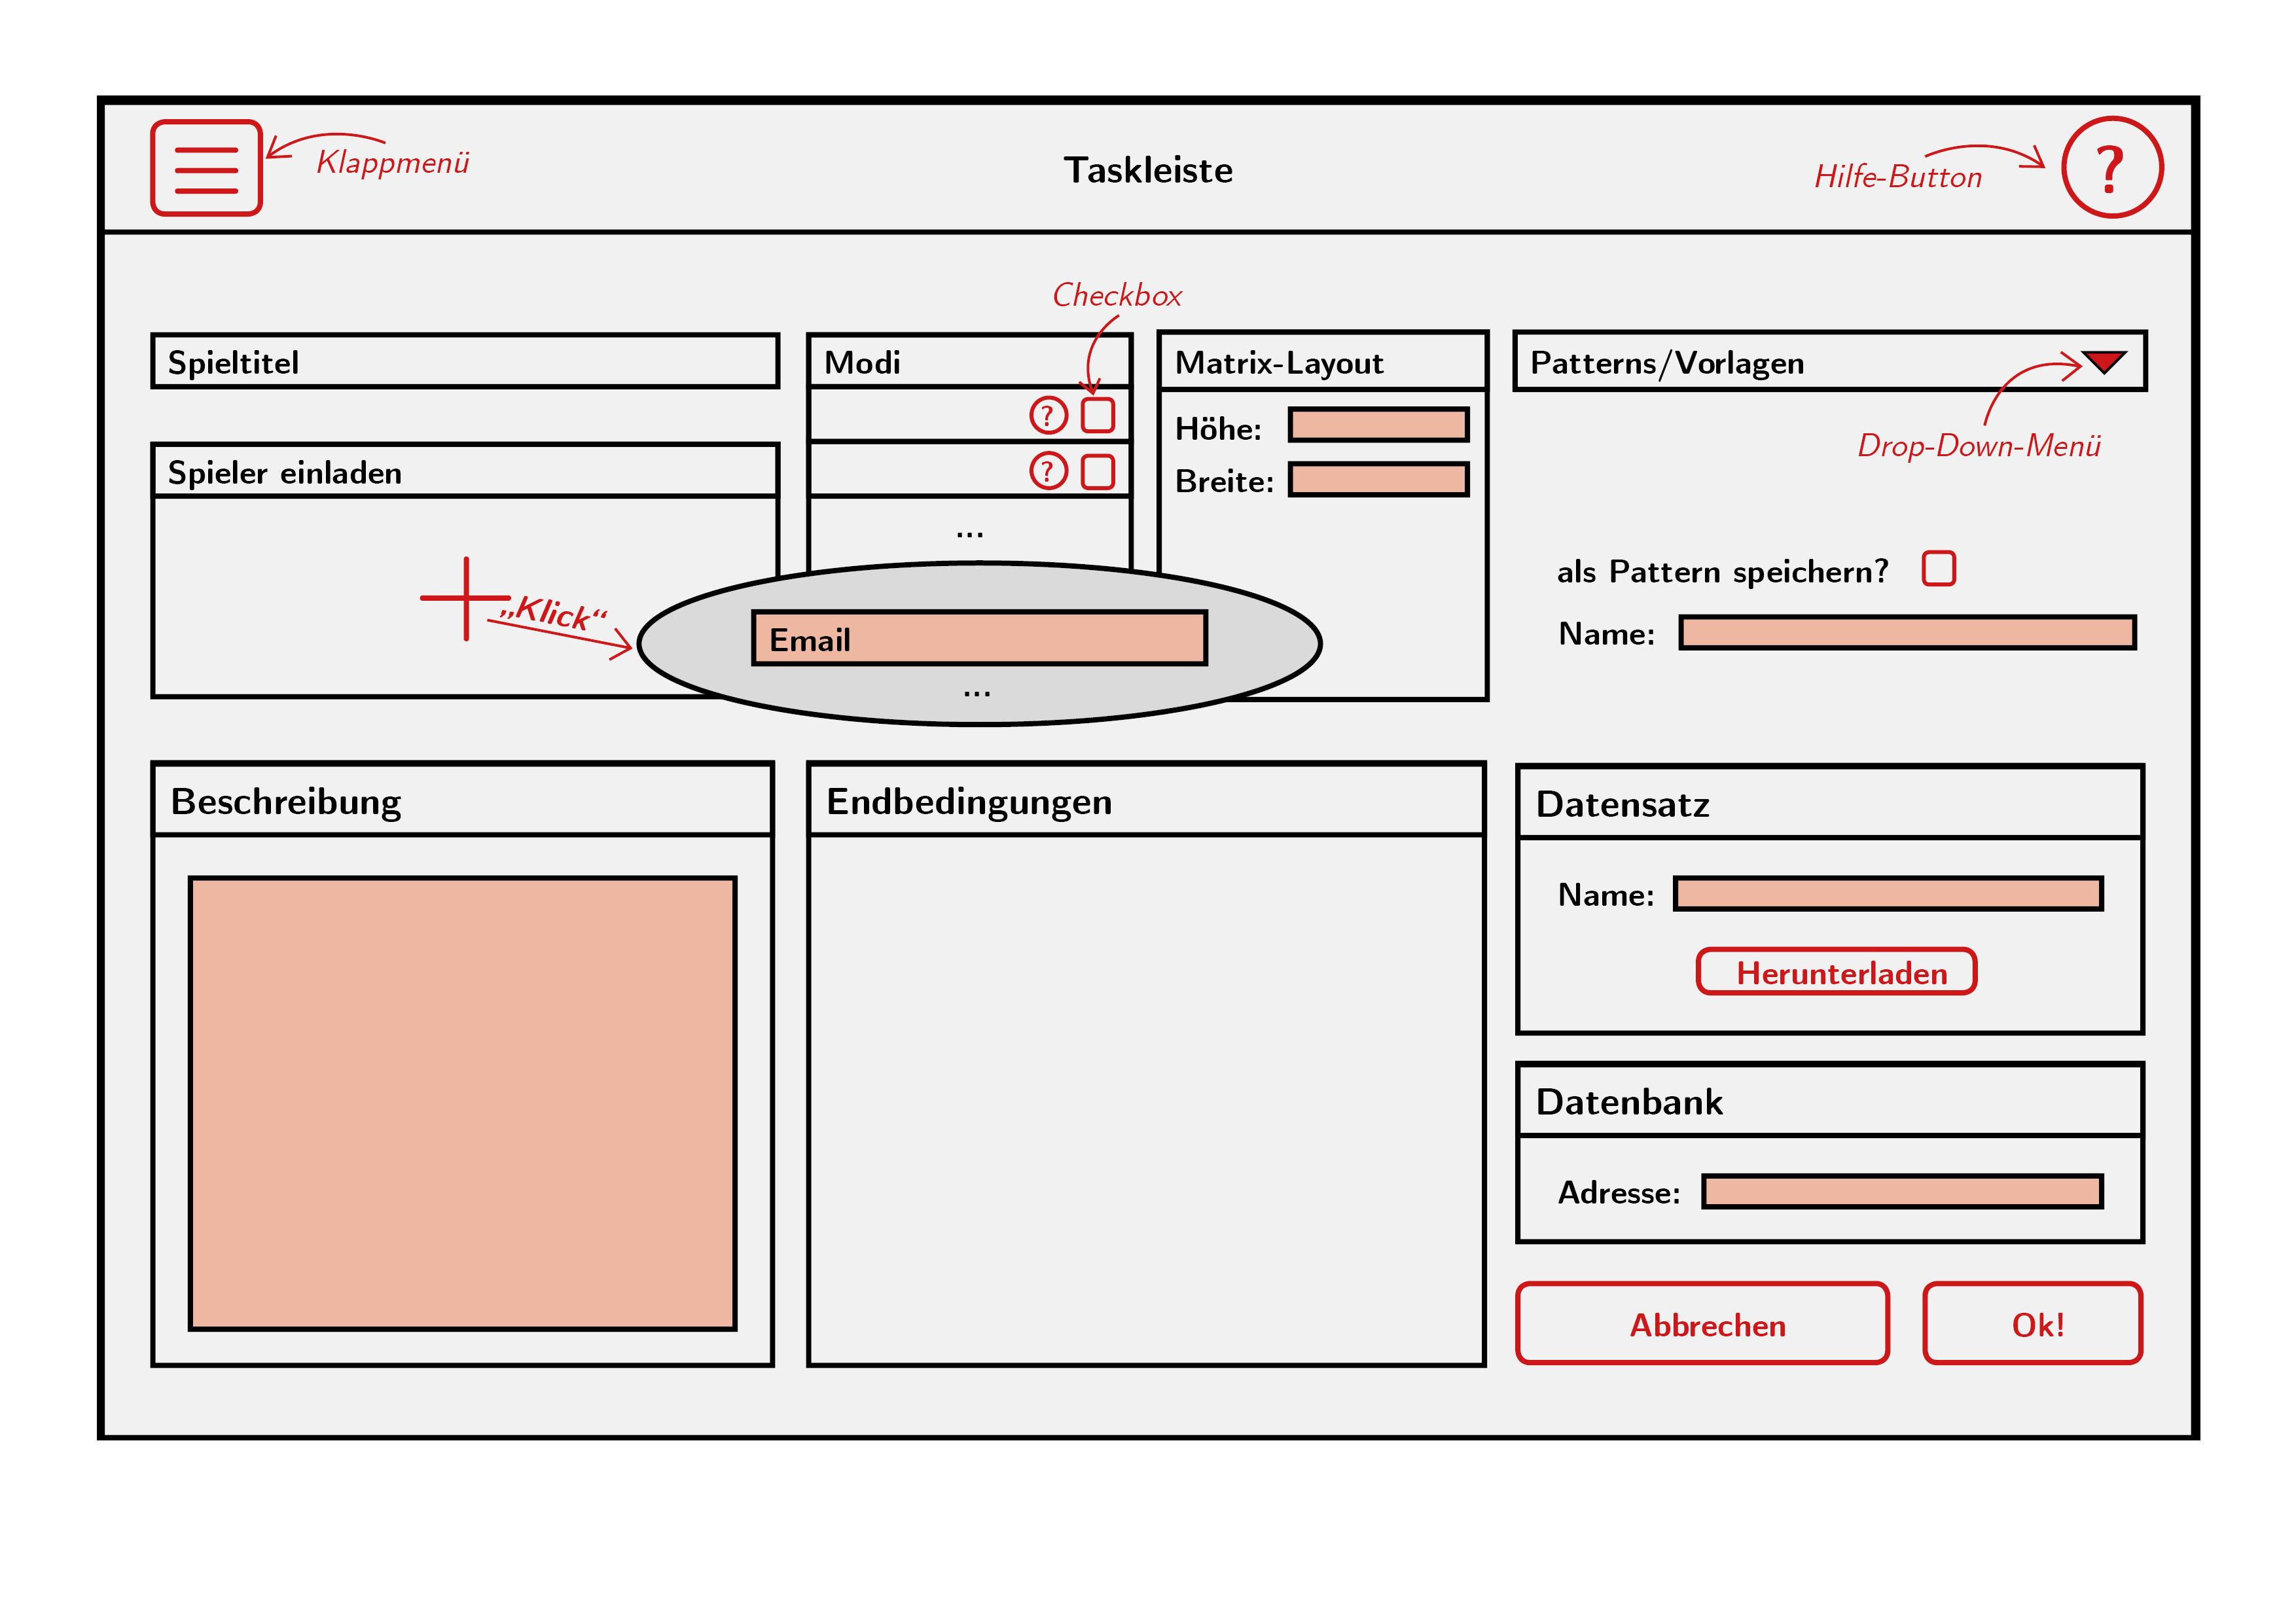
\includegraphics[width=\textwidth]{../pictures/Spielerstellung.jpg}

    \section{Spieler-Übersicht}
    \label{fig:Spieler-Übersicht}
    \centering
    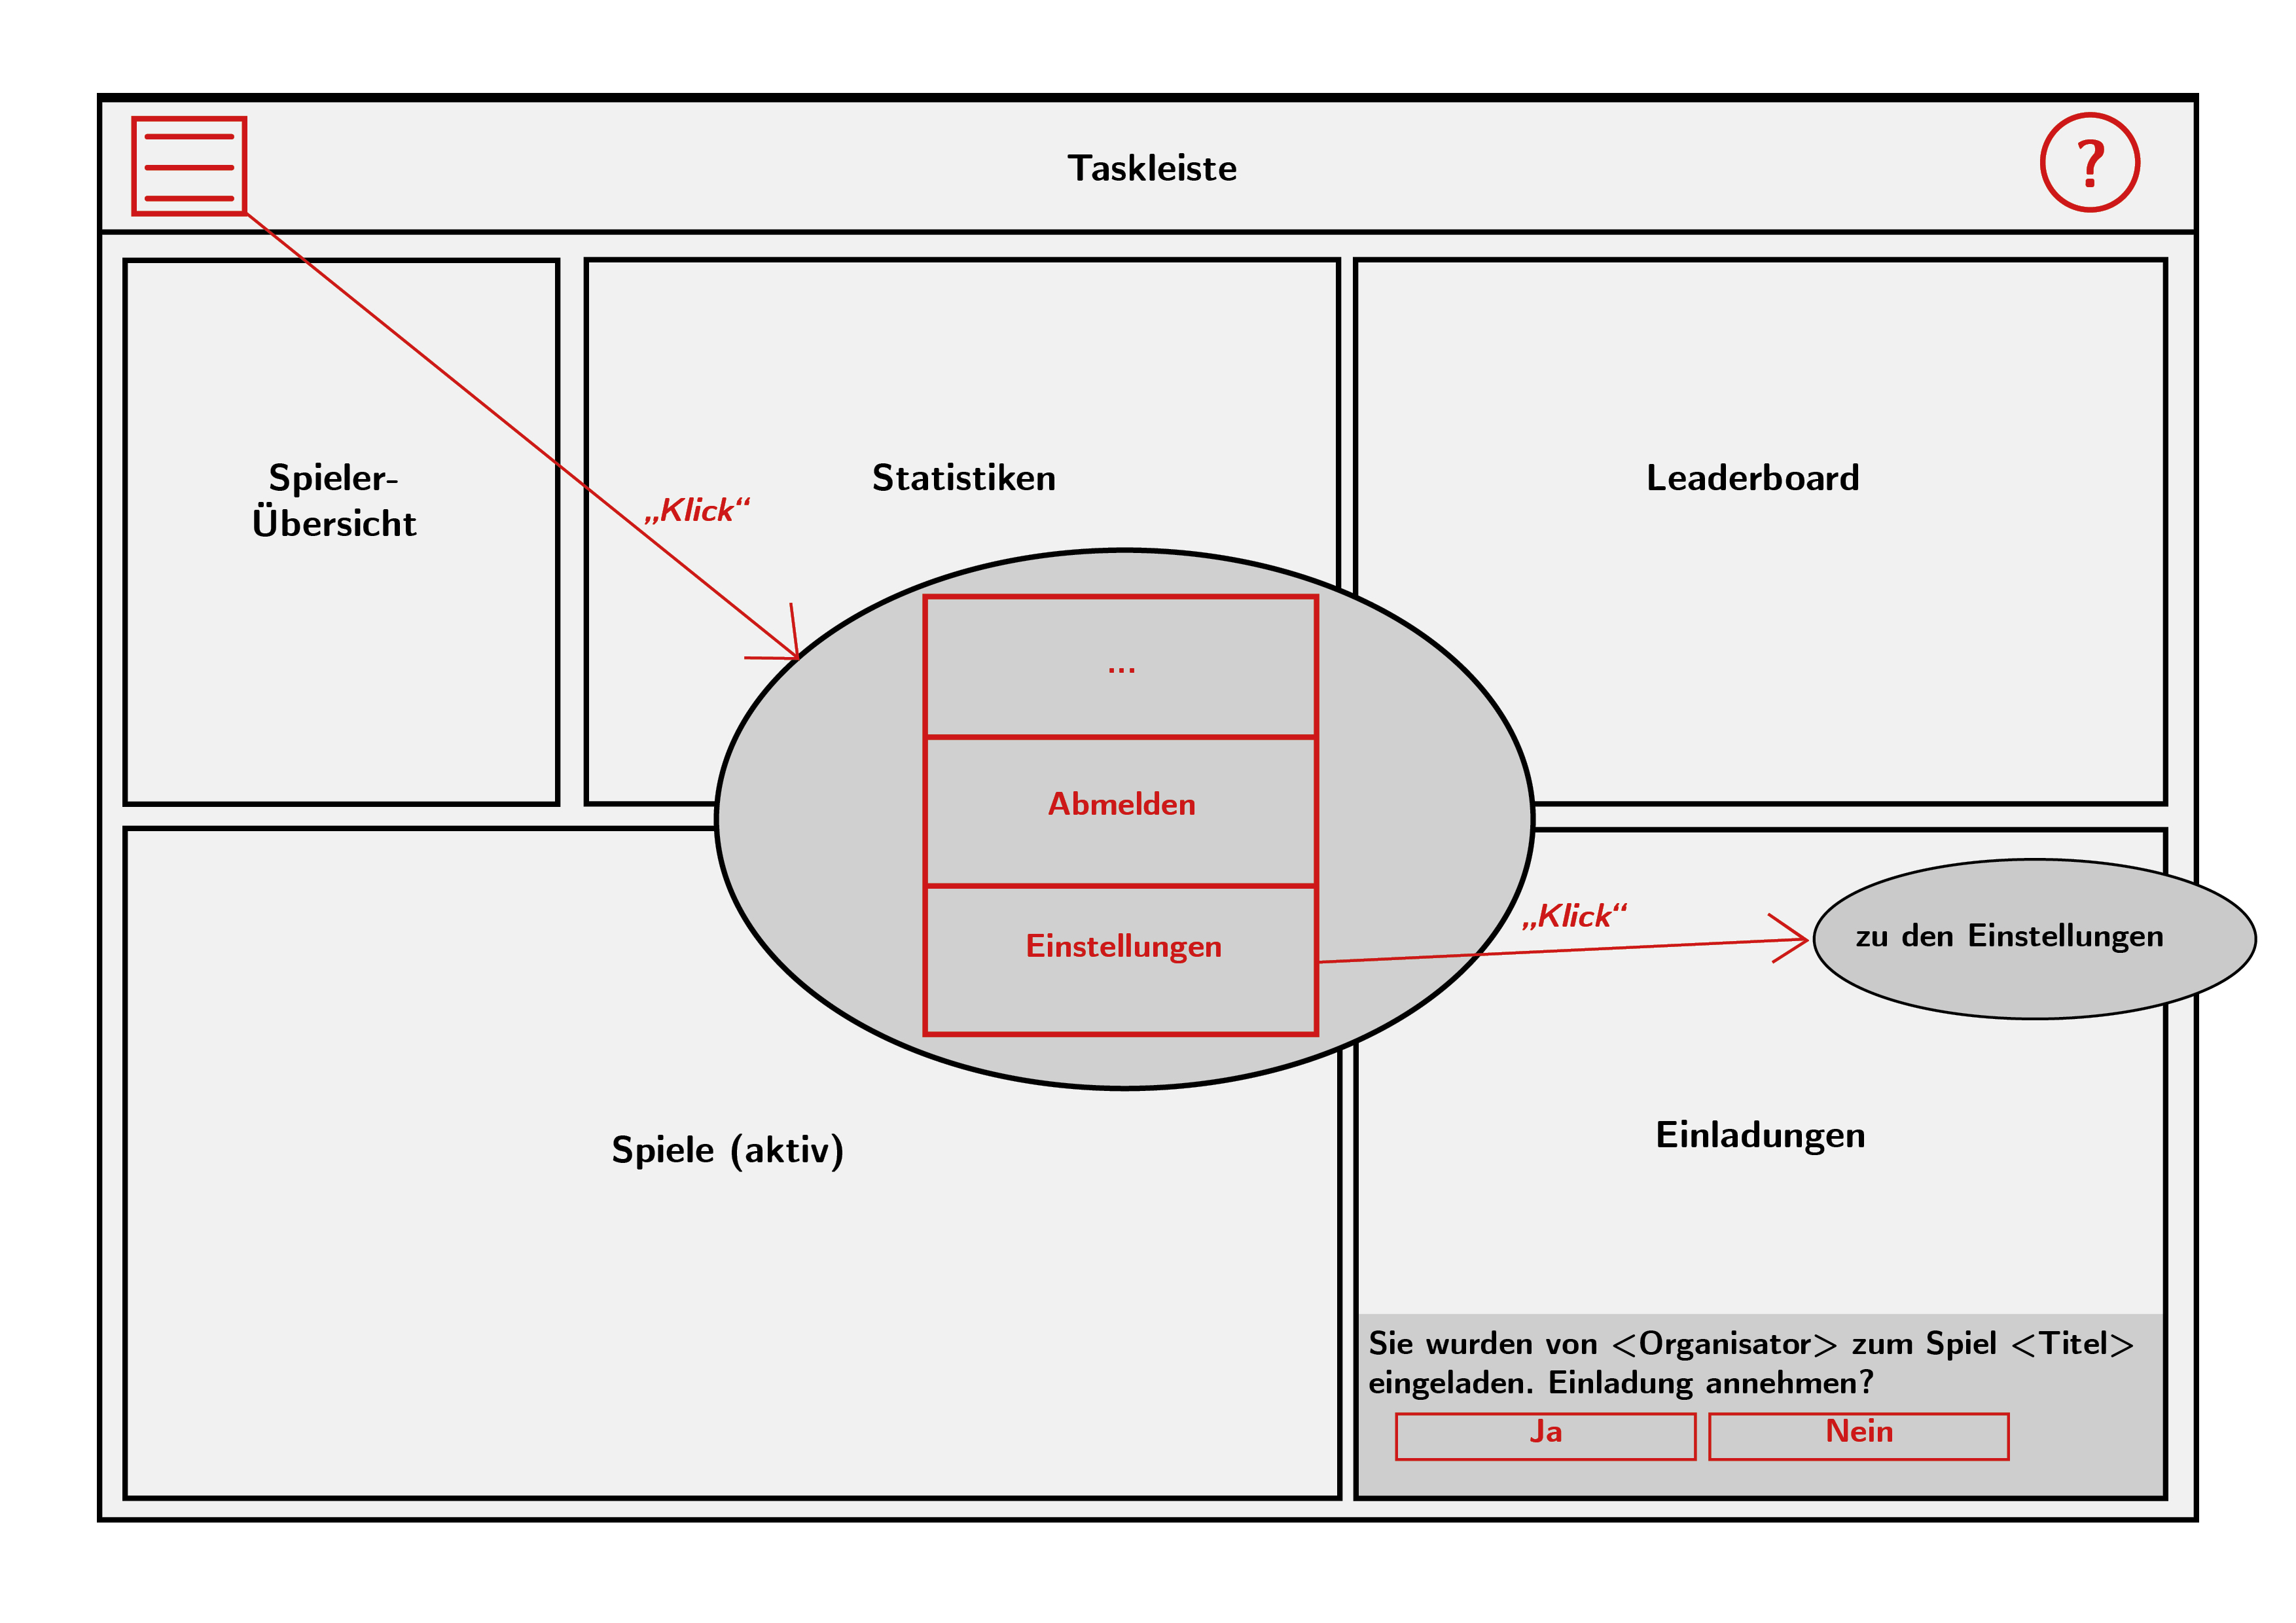
\includegraphics[width=\textwidth]{../pictures/5_Spieler.jpg}

    \section{Spiel}
    \subsection{Matrix Select}
    \centering
    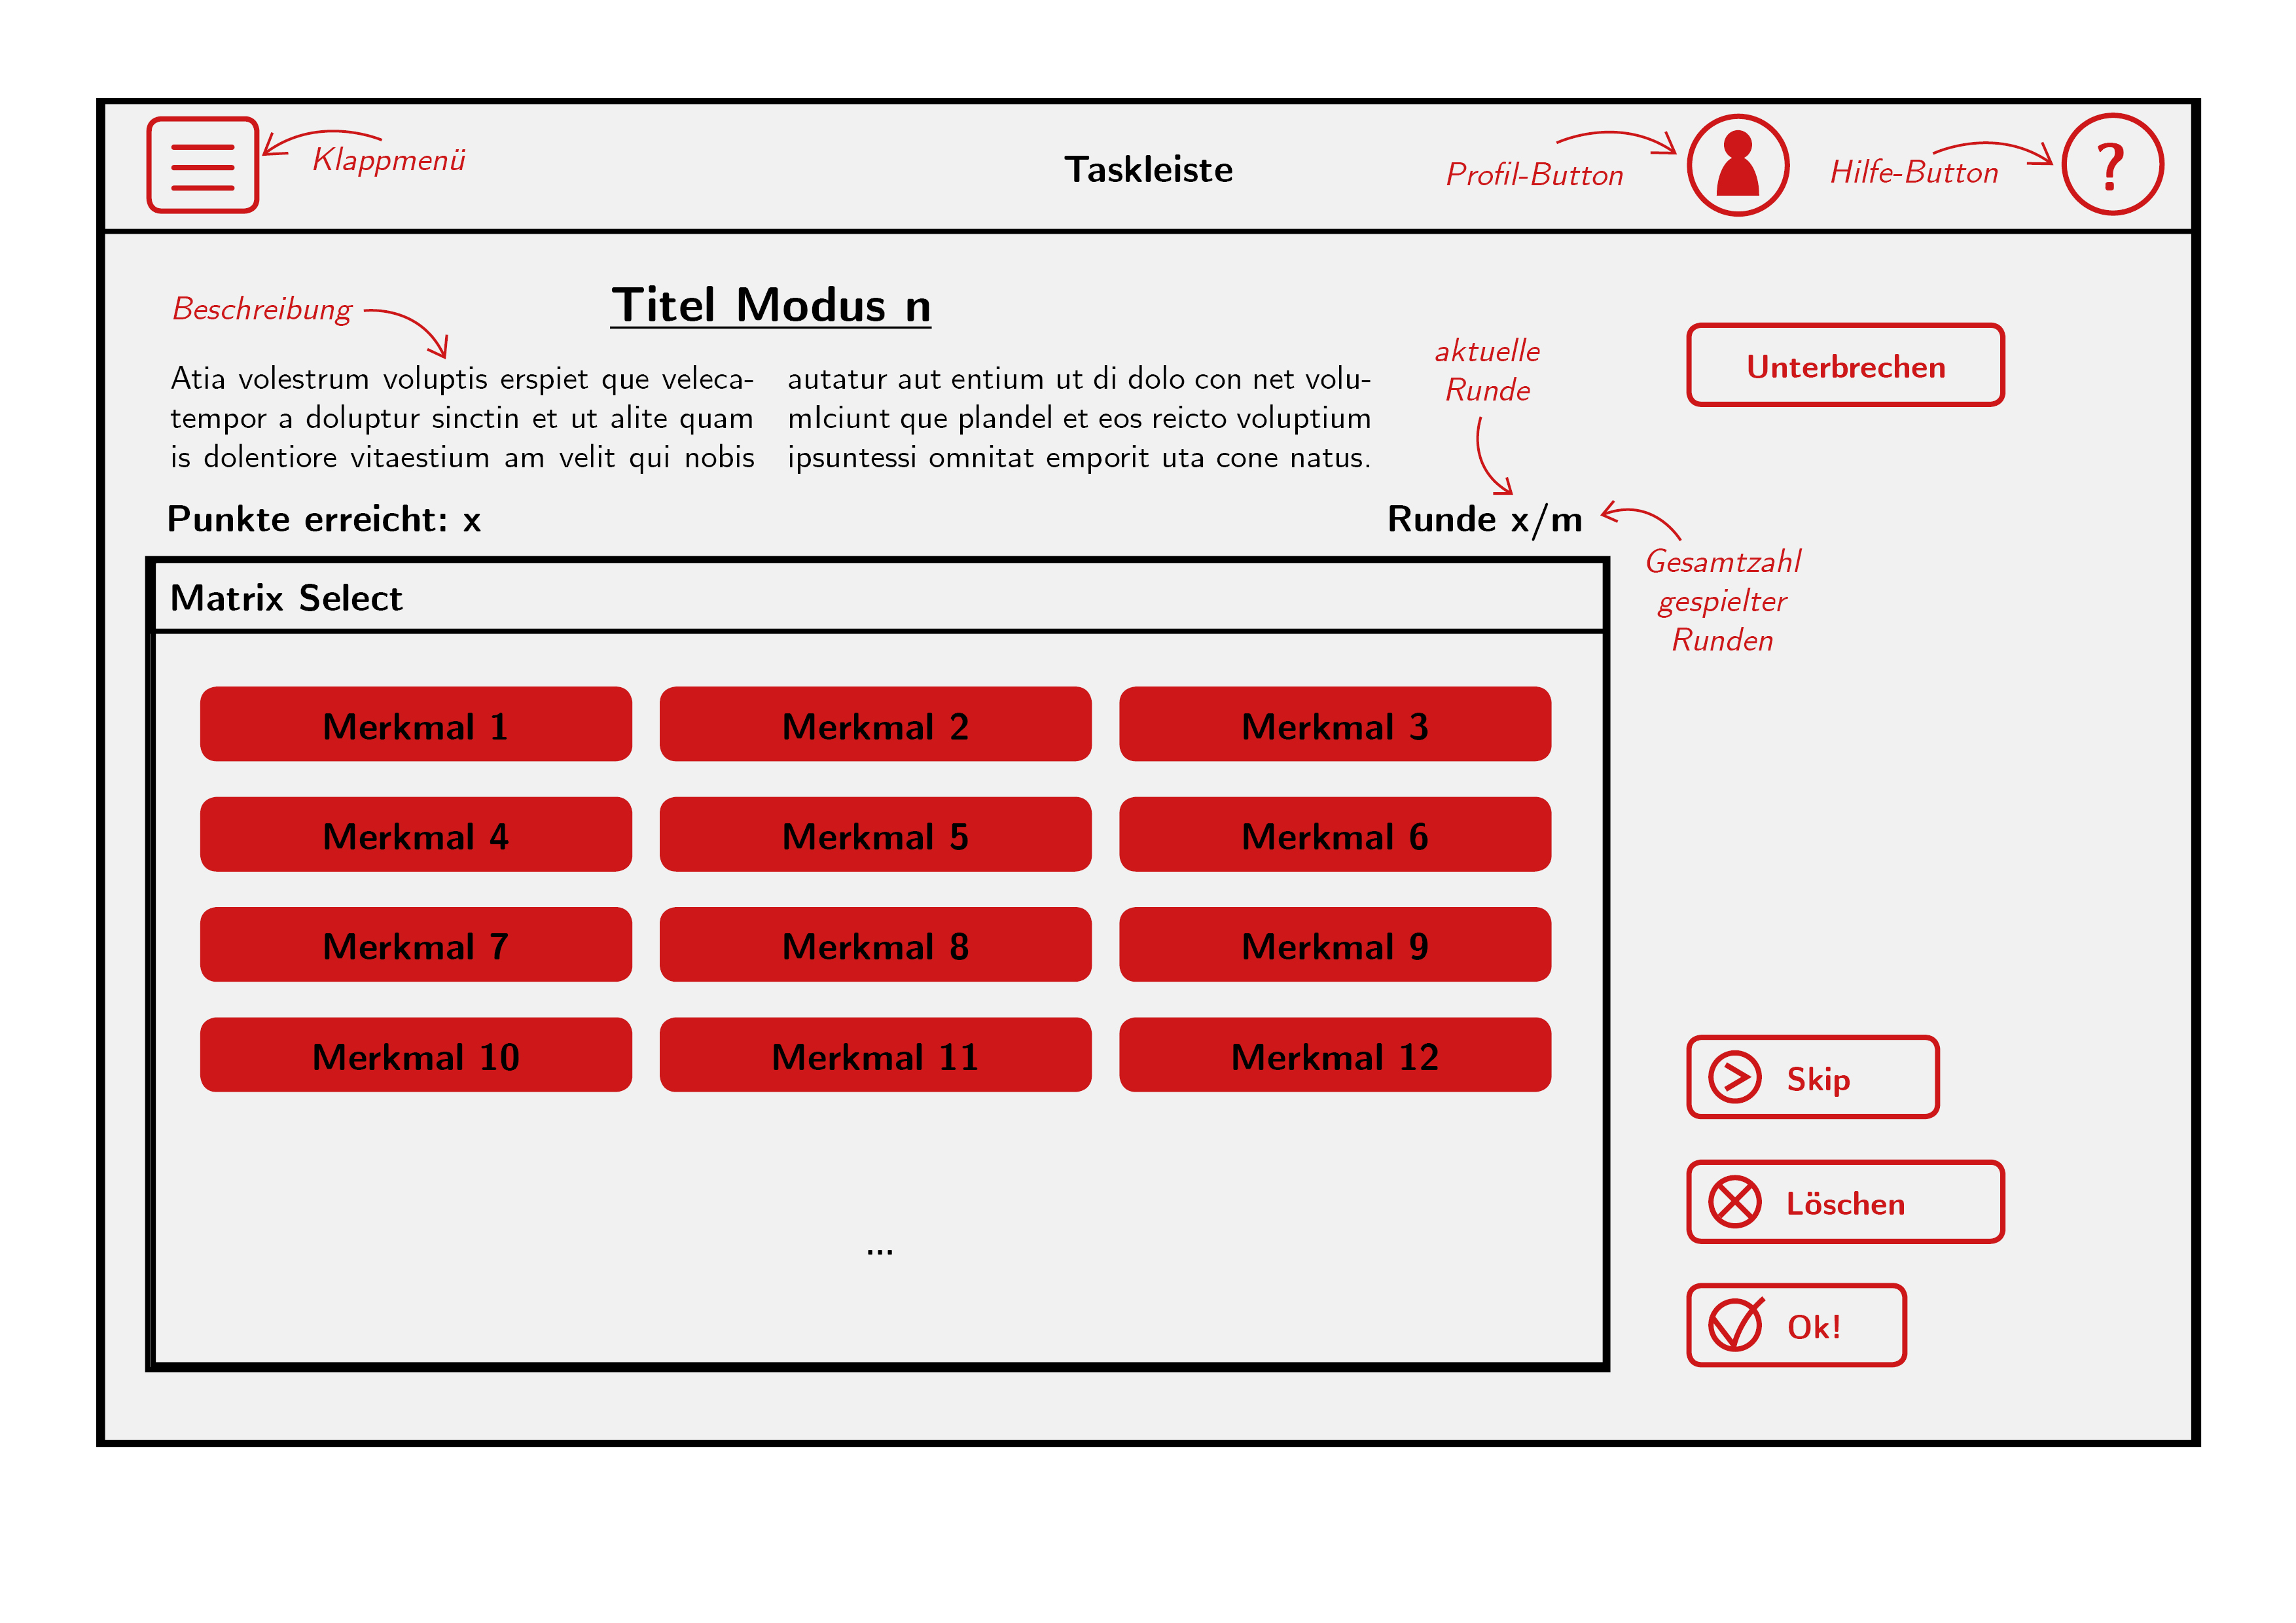
\includegraphics[width=\textwidth]{../pictures/MatrixSelect.jpg}
    \subsection{Binär Select}
    \centering
    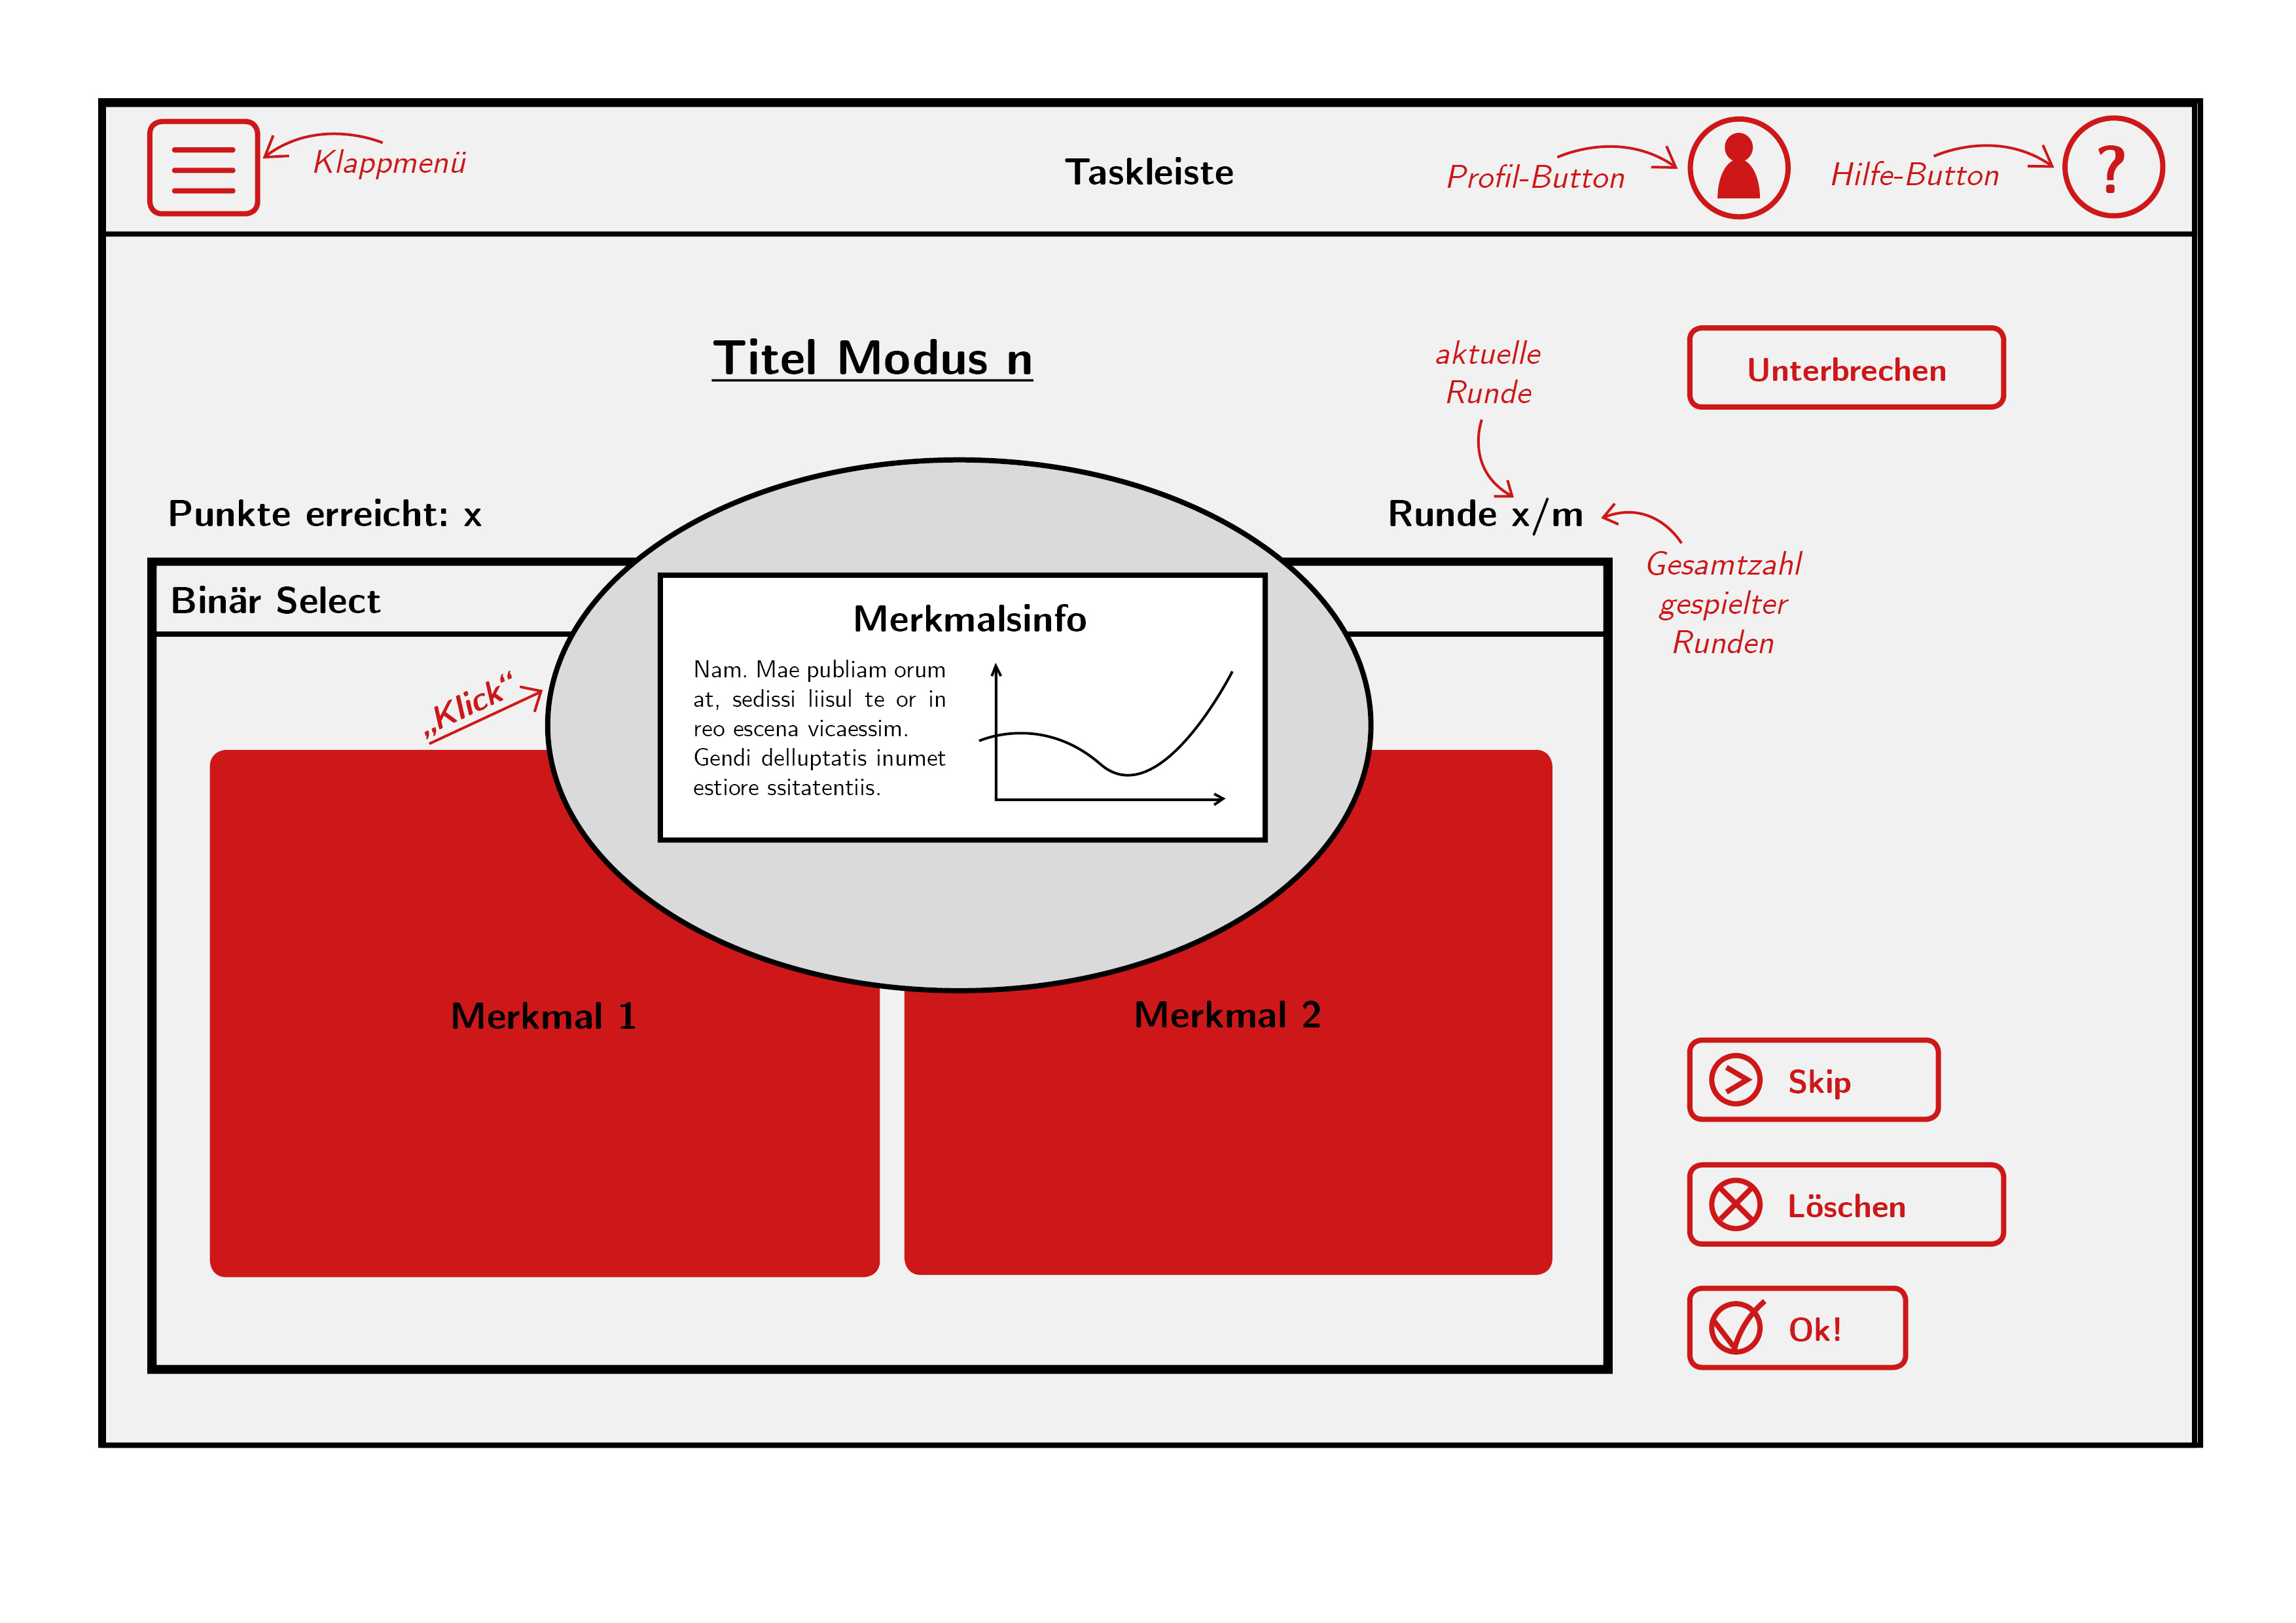
\includegraphics[width=\textwidth]{../pictures/BinSelect.jpg}

    \clearpage


    \chapter{Glossar}
    \printglossary
    
\end{document}
